% Options for packages loaded elsewhere
\PassOptionsToPackage{unicode}{hyperref}
\PassOptionsToPackage{hyphens}{url}
\PassOptionsToPackage{dvipsnames,svgnames,x11names}{xcolor}
%
\documentclass[
  12pt,
  letterpaper,
]{book}

\usepackage{amsmath,amssymb}
\usepackage{iftex}
\ifPDFTeX
  \usepackage[T1]{fontenc}
  \usepackage[utf8]{inputenc}
  \usepackage{textcomp} % provide euro and other symbols
\else % if luatex or xetex
  \usepackage{unicode-math}
  \defaultfontfeatures{Scale=MatchLowercase}
  \defaultfontfeatures[\rmfamily]{Ligatures=TeX,Scale=1}
\fi
\usepackage{lmodern}
\ifPDFTeX\else  
    % xetex/luatex font selection
  \setmainfont[]{Latin Modern Roman}
  \setsansfont[]{Latin Modern Sans}
  \setmonofont[]{Latin Modern Mono}
\fi
% Use upquote if available, for straight quotes in verbatim environments
\IfFileExists{upquote.sty}{\usepackage{upquote}}{}
\IfFileExists{microtype.sty}{% use microtype if available
  \usepackage[]{microtype}
  \UseMicrotypeSet[protrusion]{basicmath} % disable protrusion for tt fonts
}{}
\makeatletter
\@ifundefined{KOMAClassName}{% if non-KOMA class
  \IfFileExists{parskip.sty}{%
    \usepackage{parskip}
  }{% else
    \setlength{\parindent}{0pt}
    \setlength{\parskip}{6pt plus 2pt minus 1pt}}
}{% if KOMA class
  \KOMAoptions{parskip=half}}
\makeatother
\usepackage{xcolor}
\usepackage[margin=1in]{geometry}
\setlength{\emergencystretch}{3em} % prevent overfull lines
\setcounter{secnumdepth}{3}
% Make \paragraph and \subparagraph free-standing
\ifx\paragraph\undefined\else
  \let\oldparagraph\paragraph
  \renewcommand{\paragraph}[1]{\oldparagraph{#1}\mbox{}}
\fi
\ifx\subparagraph\undefined\else
  \let\oldsubparagraph\subparagraph
  \renewcommand{\subparagraph}[1]{\oldsubparagraph{#1}\mbox{}}
\fi

\usepackage{color}
\usepackage{fancyvrb}
\newcommand{\VerbBar}{|}
\newcommand{\VERB}{\Verb[commandchars=\\\{\}]}
\DefineVerbatimEnvironment{Highlighting}{Verbatim}{commandchars=\\\{\}}
% Add ',fontsize=\small' for more characters per line
\newenvironment{Shaded}{}{}
\newcommand{\AlertTok}[1]{\textcolor[rgb]{1.00,0.33,0.33}{\textbf{#1}}}
\newcommand{\AnnotationTok}[1]{\textcolor[rgb]{0.42,0.45,0.49}{#1}}
\newcommand{\AttributeTok}[1]{\textcolor[rgb]{0.84,0.23,0.29}{#1}}
\newcommand{\BaseNTok}[1]{\textcolor[rgb]{0.00,0.36,0.77}{#1}}
\newcommand{\BuiltInTok}[1]{\textcolor[rgb]{0.84,0.23,0.29}{#1}}
\newcommand{\CharTok}[1]{\textcolor[rgb]{0.01,0.18,0.38}{#1}}
\newcommand{\CommentTok}[1]{\textcolor[rgb]{0.42,0.45,0.49}{#1}}
\newcommand{\CommentVarTok}[1]{\textcolor[rgb]{0.42,0.45,0.49}{#1}}
\newcommand{\ConstantTok}[1]{\textcolor[rgb]{0.00,0.36,0.77}{#1}}
\newcommand{\ControlFlowTok}[1]{\textcolor[rgb]{0.84,0.23,0.29}{#1}}
\newcommand{\DataTypeTok}[1]{\textcolor[rgb]{0.84,0.23,0.29}{#1}}
\newcommand{\DecValTok}[1]{\textcolor[rgb]{0.00,0.36,0.77}{#1}}
\newcommand{\DocumentationTok}[1]{\textcolor[rgb]{0.42,0.45,0.49}{#1}}
\newcommand{\ErrorTok}[1]{\textcolor[rgb]{1.00,0.33,0.33}{\underline{#1}}}
\newcommand{\ExtensionTok}[1]{\textcolor[rgb]{0.84,0.23,0.29}{\textbf{#1}}}
\newcommand{\FloatTok}[1]{\textcolor[rgb]{0.00,0.36,0.77}{#1}}
\newcommand{\FunctionTok}[1]{\textcolor[rgb]{0.44,0.26,0.76}{#1}}
\newcommand{\ImportTok}[1]{\textcolor[rgb]{0.01,0.18,0.38}{#1}}
\newcommand{\InformationTok}[1]{\textcolor[rgb]{0.42,0.45,0.49}{#1}}
\newcommand{\KeywordTok}[1]{\textcolor[rgb]{0.84,0.23,0.29}{#1}}
\newcommand{\NormalTok}[1]{\textcolor[rgb]{0.14,0.16,0.18}{#1}}
\newcommand{\OperatorTok}[1]{\textcolor[rgb]{0.14,0.16,0.18}{#1}}
\newcommand{\OtherTok}[1]{\textcolor[rgb]{0.44,0.26,0.76}{#1}}
\newcommand{\PreprocessorTok}[1]{\textcolor[rgb]{0.84,0.23,0.29}{#1}}
\newcommand{\RegionMarkerTok}[1]{\textcolor[rgb]{0.42,0.45,0.49}{#1}}
\newcommand{\SpecialCharTok}[1]{\textcolor[rgb]{0.00,0.36,0.77}{#1}}
\newcommand{\SpecialStringTok}[1]{\textcolor[rgb]{0.01,0.18,0.38}{#1}}
\newcommand{\StringTok}[1]{\textcolor[rgb]{0.01,0.18,0.38}{#1}}
\newcommand{\VariableTok}[1]{\textcolor[rgb]{0.89,0.38,0.04}{#1}}
\newcommand{\VerbatimStringTok}[1]{\textcolor[rgb]{0.01,0.18,0.38}{#1}}
\newcommand{\WarningTok}[1]{\textcolor[rgb]{1.00,0.33,0.33}{#1}}

\providecommand{\tightlist}{%
  \setlength{\itemsep}{0pt}\setlength{\parskip}{0pt}}\usepackage{longtable,booktabs,array}
\usepackage{calc} % for calculating minipage widths
% Correct order of tables after \paragraph or \subparagraph
\usepackage{etoolbox}
\makeatletter
\patchcmd\longtable{\par}{\if@noskipsec\mbox{}\fi\par}{}{}
\makeatother
% Allow footnotes in longtable head/foot
\IfFileExists{footnotehyper.sty}{\usepackage{footnotehyper}}{\usepackage{footnote}}
\makesavenoteenv{longtable}
\usepackage{graphicx}
\makeatletter
\def\maxwidth{\ifdim\Gin@nat@width>\linewidth\linewidth\else\Gin@nat@width\fi}
\def\maxheight{\ifdim\Gin@nat@height>\textheight\textheight\else\Gin@nat@height\fi}
\makeatother
% Scale images if necessary, so that they will not overflow the page
% margins by default, and it is still possible to overwrite the defaults
% using explicit options in \includegraphics[width, height, ...]{}
\setkeys{Gin}{width=\maxwidth,height=\maxheight,keepaspectratio}
% Set default figure placement to htbp
\makeatletter
\def\fps@figure{htbp}
\makeatother

\usepackage{amsmath}
\usepackage{amssymb}
\usepackage{amsthm}
\makeatletter
\@ifpackageloaded{tcolorbox}{}{\usepackage[skins,breakable]{tcolorbox}}
\@ifpackageloaded{fontawesome5}{}{\usepackage{fontawesome5}}
\definecolor{quarto-callout-color}{HTML}{909090}
\definecolor{quarto-callout-note-color}{HTML}{0758E5}
\definecolor{quarto-callout-important-color}{HTML}{CC1914}
\definecolor{quarto-callout-warning-color}{HTML}{EB9113}
\definecolor{quarto-callout-tip-color}{HTML}{00A047}
\definecolor{quarto-callout-caution-color}{HTML}{FC5300}
\definecolor{quarto-callout-color-frame}{HTML}{acacac}
\definecolor{quarto-callout-note-color-frame}{HTML}{4582ec}
\definecolor{quarto-callout-important-color-frame}{HTML}{d9534f}
\definecolor{quarto-callout-warning-color-frame}{HTML}{f0ad4e}
\definecolor{quarto-callout-tip-color-frame}{HTML}{02b875}
\definecolor{quarto-callout-caution-color-frame}{HTML}{fd7e14}
\makeatother
\makeatletter
\makeatother
\makeatletter
\@ifpackageloaded{bookmark}{}{\usepackage{bookmark}}
\makeatother
\makeatletter
\@ifpackageloaded{caption}{}{\usepackage{caption}}
\AtBeginDocument{%
\ifdefined\contentsname
  \renewcommand*\contentsname{Table des matières}
\else
  \newcommand\contentsname{Table des matières}
\fi
\ifdefined\listfigurename
  \renewcommand*\listfigurename{Liste des Figures}
\else
  \newcommand\listfigurename{Liste des Figures}
\fi
\ifdefined\listtablename
  \renewcommand*\listtablename{Liste des Tables}
\else
  \newcommand\listtablename{Liste des Tables}
\fi
\ifdefined\figurename
  \renewcommand*\figurename{Figure}
\else
  \newcommand\figurename{Figure}
\fi
\ifdefined\tablename
  \renewcommand*\tablename{Table}
\else
  \newcommand\tablename{Table}
\fi
}
\@ifpackageloaded{float}{}{\usepackage{float}}
\floatstyle{ruled}
\@ifundefined{c@chapter}{\newfloat{codelisting}{h}{lop}}{\newfloat{codelisting}{h}{lop}[chapter]}
\floatname{codelisting}{Listing}
\newcommand*\listoflistings{\listof{codelisting}{Liste des Listings}}
\usepackage{amsthm}
\theoremstyle{remark}
\AtBeginDocument{\renewcommand*{\proofname}{Preuve}}
\newtheorem*{remark}{Remarque}
\newtheorem*{solution}{Solution}
\makeatother
\makeatletter
\@ifpackageloaded{caption}{}{\usepackage{caption}}
\@ifpackageloaded{subcaption}{}{\usepackage{subcaption}}
\makeatother
\makeatletter
\@ifpackageloaded{tcolorbox}{}{\usepackage[skins,breakable]{tcolorbox}}
\makeatother
\makeatletter
\@ifundefined{shadecolor}{\definecolor{shadecolor}{rgb}{.97, .97, .97}}
\makeatother
\makeatletter
\makeatother
\makeatletter
\makeatother
\ifLuaTeX
\usepackage[bidi=basic]{babel}
\else
\usepackage[bidi=default]{babel}
\fi
\babelprovide[main,import]{french}
% get rid of language-specific shorthands (see #6817):
\let\LanguageShortHands\languageshorthands
\def\languageshorthands#1{}
\ifLuaTeX
  \usepackage{selnolig}  % disable illegal ligatures
\fi
\usepackage[]{biblatex}
\IfFileExists{bookmark.sty}{\usepackage{bookmark}}{\usepackage{hyperref}}
\IfFileExists{xurl.sty}{\usepackage{xurl}}{} % add URL line breaks if available
\urlstyle{same} % disable monospaced font for URLs
\hypersetup{
  pdftitle={MAT-2904 : Complément d'analyse},
  pdfauthor={Jérôme Soucy},
  pdflang={fr},
  colorlinks=true,
  linkcolor={blue},
  filecolor={Maroon},
  citecolor={Blue},
  urlcolor={blue},
  pdfcreator={LaTeX via pandoc}}

\title{MAT-2904 : Complément d'analyse}
\author{Jérôme Soucy}
\date{}

\begin{document}
\frontmatter
\maketitle
\ifdefined\Shaded\renewenvironment{Shaded}{\begin{tcolorbox}[boxrule=0pt, breakable, interior hidden, borderline west={3pt}{0pt}{shadecolor}, frame hidden, sharp corners, enhanced]}{\end{tcolorbox}}\fi

\renewcommand*\contentsname{Table des matières}
{
\hypersetup{linkcolor=}
\setcounter{tocdepth}{2}
\tableofcontents
}
\listoffigures
\listoftables
\mainmatter
\bookmarksetup{startatroot}

\hypertarget{pruxe9sentation}{%
\chapter*{Présentation}\label{pruxe9sentation}}
\addcontentsline{toc}{chapter}{Présentation}

\markboth{Présentation}{Présentation}

Bienvenue sur un site web complémentaire au site monPortail du cours
\textbf{MAT-2904 : Complément d'analyse}, à l'Université Laval.

Ce site contient principalement des séries d'exercices conçues pour
accompagner les étudiants et étudiantes dans le cours. Chaque série
d'exercices est soigneusement élaborée pour approfondir votre
compréhension des concepts clés et vous préparer aux évaluations.

\hypertarget{les-fonctions-exponentielles-et-logarithmiques}{%
\section*{Les fonctions exponentielles et
logarithmiques}\label{les-fonctions-exponentielles-et-logarithmiques}}
\addcontentsline{toc}{section}{Les fonctions exponentielles et
logarithmiques}

\markright{Les fonctions exponentielles et logarithmiques}

Ce document vous invite à explorer en profondeur les fonctions
exponentielles et logarithmiques, des outils mathématiques essentiels
tant en théorie qu'en applications pratiques. À travers onze exercices
soigneusement structurés, vous allez découvrir les multiples facettes de
ces fonctions.

Nous commençons par des exercices techniques de résolution d'équations
exponentielles, avant d'aborder des problèmes plus théoriques qui vous
feront découvrir les propriétés fondamentales de la fonction
exponentielle, notamment son unicité comme solution de l'équation
différentielle f'=f.

Le document intègre également des applications concrètes avec des
problèmes d'intérêts composés et de croissance de populations
bactériennes, illustrant ainsi l'utilité pratique de ces fonctions.

Nous terminons par une exploration rigoureuse de la définition du nombre
e, démontrant comment ce nombre fondamental émerge naturellement des
limites de suites. Les solutions détaillées vous guideront à travers les
raisonnements mathématiques nécessaires pour maîtriser ces concepts clés
de l'analyse mathématique.

\hypertarget{les-fonctions-puissances}{%
\section*{Les fonctions puissances}\label{les-fonctions-puissances}}
\addcontentsline{toc}{section}{Les fonctions puissances}

\markright{Les fonctions puissances}

Ce document vous propose une exploration approfondie des fonctions
puissances, un concept fondamental en analyse mathématique. À travers
onze exercices progressifs, vous allez consolider votre compréhension
des propriétés algébriques et analytiques de ces fonctions.

Nous commençons par établir les propriétés fondamentales des puissances
en utilisant la définition \(x^{\alpha} = e^{\alpha \log x}\), puis nous
abordons des questions plus subtiles comme la rationalité des puissances
de nombres irrationnels.

Le document vous guide ensuite vers l'étude des dérivées des fonctions
puissances, avec une attention particulière portée à l'analyse complète
de la fonction racine cubique.

Les exercices culminent avec des applications pratiques :

\begin{itemize}
\tightlist
\item
  Calcul de limites
\item
  Résolution d'équations et d'inéquations
\item
  Calcul d'intégrales faisant intervenir des puissances réelles
\end{itemize}

Chaque exercice est accompagné d'une solution détaillée et, lorsque
pertinent, de représentations graphiques pour faciliter votre
compréhension.

\hypertarget{lintuxe9grale-de-riemann}{%
\section*{L'intégrale de Riemann}\label{lintuxe9grale-de-riemann}}
\addcontentsline{toc}{section}{L'intégrale de Riemann}

\markright{L'intégrale de Riemann}

Ce document vous propose une série d'exercices approfondis sur
l'intégrale de Riemann, un concept fondamental en analyse mathématique.
Vous y trouverez six questions (incluant plusieurs sous-questions) qui
vous permettront de maîtriser différentes techniques d'intégration et de
comprendre leurs applications.

La première partie vous invite à pratiquer l'intégration indéfinie à
travers douze cas différents, chacun nécessitant des techniques
spécifiques comme :

\begin{itemize}
\tightlist
\item
  Les changements de variables
\item
  L'intégration par parties
\item
  La décomposition en fractions partielles
\end{itemize}

Les exercices suivants vous amènent vers des concepts plus avancés :

\begin{itemize}
\tightlist
\item
  Le calcul d'intégrales définies, y compris avec des bornes infinies
\item
  Le calcul d'aire entre des courbes
\item
  Une démonstration rigoureuse par la méthode de Riemann
\item
  Des questions plus théoriques sur les propriétés des fonctions
  impaires dans l'intégration
\end{itemize}

Chaque exercice est accompagné d'une solution détaillée qui vous permet
de comprendre pas à pas la méthode de résolution.

\hypertarget{les-fonctions-hyperboliques}{%
\section*{Les fonctions
hyperboliques}\label{les-fonctions-hyperboliques}}
\addcontentsline{toc}{section}{Les fonctions hyperboliques}

\markright{Les fonctions hyperboliques}

Dans cette série d'exercices sur les fonctions hyperboliques, nous
explorons d'abord les fonctions de base sinh, cosh et tanh, en mettant
l'accent sur leurs graphiques et leurs propriétés fondamentales. Une
attention particulière est portée à la fonction tanh et sa réciproque
arctanh, où nous démontrons notamment la formule importante reliant
arctanh(x) au logarithme naturel. Les graphiques sont systématiquement
tracés pour visualiser le comportement de ces fonctions.

La série progresse ensuite vers des aspects plus théoriques avec la
démonstration d'identités hyperboliques importantes, comme la formule
d'addition pour cosh(x+y). Ces identités sont suivies d'exercices de
résolution d'équations impliquant sinh et cosh, montrant comment ces
fonctions sont interconnectées par des relations fondamentales comme
cosh²(x) - sinh²(x) = 1. Une partie intéressante de la série est
consacrée à la comparaison graphique de sinh et cosh, nous permettant de
mieux comprendre leurs comportements respectifs.

La série se termine par une application concrète et fascinante : l'étude
de la chaînette, qui représente la forme que prend un câble suspendu
sous son propre poids. Ce problème pratique nous montre comment les
fonctions hyperboliques apparaissent naturellement dans des situations
physiques réelles, illustrant ainsi leur importance au-delà des
mathématiques pures.

\hypertarget{licence-et-attributions}{%
\section*{Licence et attributions}\label{licence-et-attributions}}
\addcontentsline{toc}{section}{Licence et attributions}

\markright{Licence et attributions}

Ce site et son contenu sont mis à disposition sous licence Creative
Commons Attribution - Pas d'Utilisation Commerciale (CC BY-NC).

\begin{tcolorbox}[enhanced jigsaw, titlerule=0mm, opacityback=0, opacitybacktitle=0.6, colbacktitle=quarto-callout-note-color!10!white, breakable, arc=.35mm, title=\textcolor{quarto-callout-note-color}{\faInfo}\hspace{0.5em}{Droits d'utilisation}, colframe=quarto-callout-note-color-frame, toptitle=1mm, bottomrule=.15mm, bottomtitle=1mm, rightrule=.15mm, toprule=.15mm, leftrule=.75mm, colback=white, left=2mm, coltitle=black]

Vous êtes libre de :

\begin{itemize}
\tightlist
\item
  Partager, copier et redistribuer le contenu
\item
  Adapter et transformer le contenu
\end{itemize}

À condition de :

\begin{itemize}
\tightlist
\item
  Créditer la source en citant l'auteur du présent document avec un lien
  vers ce site
\item
  Ne pas faire d'usage commercial du contenu
\end{itemize}

Une partie du code présenté sur ce site a été généré avec l'assistance
de l'intelligence artificielle Claude (Anthropic), tout en étant vérifié
et adapté pour garantir son exactitude et sa pertinence pédagogique.

\end{tcolorbox}

\begin{figure}

\begin{minipage}[t]{0.77\linewidth}

{\centering 

\raisebox{-\height}{


\includegraphics[width=2.60417in,height=\textheight]{by-nc.png}

}

\caption{Licence Creative Commons BY-NC}

}

\end{minipage}%
%
\begin{minipage}[t]{0.23\linewidth}

{\centering 

\raisebox{-\height}{


\includegraphics[width=0.78125in,height=\textheight]{AIA.jpg}

}

\caption{Généré avec assistance IA}

}

\end{minipage}%

\caption{\label{fig-ccIA}Certains éléments de code de ce site ont été
générés par l'IA. Vous êtes libre d'utiliser le contenu de ce site dans
la mesure où vous citez la source et n'en tirez pas de bénéfice
financier.}

\end{figure}

\part{Exercices}

\hypertarget{les-fonctions-exponentielles-et-logarithmiques-1}{%
\chapter{Les fonctions exponentielles et
logarithmiques}\label{les-fonctions-exponentielles-et-logarithmiques-1}}

\hypertarget{question-1}{%
\section{Question 1}\label{question-1}}

Résolvez les équations ci-dessous.

\begin{enumerate}
\item
  \[\exp(e^{2x+1})=e^{\pi}\]

  \begin{solution}

  \[x=\frac{-1+\log\pi}{2}\]

  \end{solution}
\item
  \[e^{3x}-e^{2x}-5e^x=0\]

  \begin{solution}

  \[x=\log\left(1+\sqrt{21}\right)-\log 2=\log\frac{1+\sqrt{21}}{2}\]

  \end{solution}
\end{enumerate}

\hypertarget{question-2}{%
\section{Question 2}\label{question-2}}

Considérons l'équation \(x^y=y^x\).

\begin{enumerate}
\item
  Vérifiez que \((x,y)=(2,4)\) et \((x,y)=(4,2)\) sont des solutions de
  cette équation.

  \begin{solution}

  Il suffit de remplacer et constater.

  \end{solution}
\item
  En étudiant le graphique de la fonction \(\dfrac{\log(x)}{x}\),
  montrez que les solutions énumérées en (a) sont les seules solutions
  telles que \(x\) et \(y\) soient des nombres naturels.

  \begin{solution}

  Voici le graphique de la fonction, que vous pouvez obtenir en faisant
  une analyse des dérivées première et seconde.

\begin{Shaded}
\begin{Highlighting}[]
\FunctionTok{library}\NormalTok{(ggplot2)}

\CommentTok{\# Création des données}
\NormalTok{x }\OtherTok{\textless{}{-}} \FunctionTok{seq}\NormalTok{(}\FloatTok{0.1}\NormalTok{, }\DecValTok{10}\NormalTok{, }\AttributeTok{length.out =} \DecValTok{1000}\NormalTok{)}
\NormalTok{y }\OtherTok{\textless{}{-}} \FunctionTok{log}\NormalTok{(x)}\SpecialCharTok{/}\NormalTok{x}

\CommentTok{\# Création du graphique}
\FunctionTok{ggplot}\NormalTok{(}\FunctionTok{data.frame}\NormalTok{(}\AttributeTok{x =}\NormalTok{ x, }\AttributeTok{y =}\NormalTok{ y), }\FunctionTok{aes}\NormalTok{(}\AttributeTok{x =}\NormalTok{ x, }\AttributeTok{y =}\NormalTok{ y)) }\SpecialCharTok{+}
  \FunctionTok{geom\_line}\NormalTok{(}\AttributeTok{color =} \StringTok{"blue"}\NormalTok{, }\AttributeTok{size =} \DecValTok{1}\NormalTok{) }\SpecialCharTok{+}
  \FunctionTok{labs}\NormalTok{(}\AttributeTok{title =} \StringTok{"Fonction ln(x)/x"}\NormalTok{,}
       \AttributeTok{x =} \StringTok{"x"}\NormalTok{,}
       \AttributeTok{y =} \StringTok{"ln(x)/x"}\NormalTok{) }\SpecialCharTok{+}
  \FunctionTok{theme\_minimal}\NormalTok{() }\SpecialCharTok{+}
  \FunctionTok{geom\_hline}\NormalTok{(}\AttributeTok{yintercept =} \DecValTok{0}\NormalTok{, }\AttributeTok{linetype =} \StringTok{"dashed"}\NormalTok{, }\AttributeTok{color =} \StringTok{"gray"}\NormalTok{) }\SpecialCharTok{+}
  \FunctionTok{geom\_vline}\NormalTok{(}\AttributeTok{xintercept =} \DecValTok{0}\NormalTok{, }\AttributeTok{linetype =} \StringTok{"dashed"}\NormalTok{, }\AttributeTok{color =} \StringTok{"gray"}\NormalTok{) }\SpecialCharTok{+}
  \FunctionTok{coord\_cartesian}\NormalTok{(}\AttributeTok{ylim =} \FunctionTok{c}\NormalTok{(}\SpecialCharTok{{-}}\FloatTok{0.5}\NormalTok{, }\FloatTok{0.4}\NormalTok{))}
\end{Highlighting}
\end{Shaded}

  \begin{figure}[H]

  {\centering \includegraphics{exercices/ExpoLog/ExpoLog_files/figure-pdf/unnamed-chunk-1-1.pdf}

  }

  \end{figure}

  On constate que l'égalité \(x^y=y^x\) est équivalente à l'égalité
  \(\frac{\log(x)}{x}=\frac{\log(y)}{y}\). Ainsi, Comme la fonction est
  strictement décroissante à partir de \(x=e\), il faut qu'une des
  valeurs se trouve avant \(e\) et une autre après \(e\). La seule
  possibilité pour une valeur entière avant \(e\) est \(2\), ce qui
  correspond à la solution trouvée en (a).

  \end{solution}
\item
  Étudiez le graphique de la fonction considérée en (b) pour déterminer
  lequel des nombres, parmi \(e^{\pi}\) et \(\pi^e\), est le plus grand.

  \begin{solution}

  On constate que l'inégalité \(x^y<y^x\) se traduit par
  \(\frac{\log(x)}{x}<\frac{\log(y)}{y}\), car la fonction \(\log\) est
  croissante. Comme la fonction \(\frac{\log(y)}{y}\) atteint son
  maximum en \(y=e\), il suit que
  \(\frac{\log(e)}{e}>\frac{\log(x)}{x}\) pour tout autre valeur de
  \(x\). Ainsi, \(\pi^e<e^{\pi}\).

  \end{solution}
\end{enumerate}

\hypertarget{question-3}{%
\section{Question 3}\label{question-3}}

Soit \(f\) une fonction vérifiant \(f(x)=f'(x)\)
\(\forall x\in\mathbb{R}\). Si \(f\) vérifie \(f(0)=1\), montrez que
\(f\) est unique.

\begin{solution}

\(f(x)=f'(x)\Rightarrow f(x)-f'(x)=0\). En multipliant de chaque côté
par \(e^{-x}\), on obtient que \(e^{-x}f(x)+f'(x)(-e^{-x})=0\). Or, le
membre de gauche de cette équation correspond à la dérivée de la
fonction \(-e^{-x}\cdot f(x)\) (appliquez la règle de dérivation d'un
produit pour vous en convaincre). Puisque la dérivée de la fonction
\(-e^{-x}f(x)\) est nulle, il existe une constante \(C\in\mathbb{R}\)
telle que \(-e^{-x}f(x)=C\). En multipliant chaque membre par \(-e^x\),
on déduit que \(f(x)=-Ce^x\). En imposant la condition \(f(0)=1\), on
déduit que \(C=-1\), d'où \(f(x)=e^x\). Ainsi, il n'y a qu'une fonction
satisfaisant simultanément les conditions \(f(x)=f'(x)\)
\(\forall x\in\mathbb{R}\) et \(f(0)=1\), à savoir la fonction
exponentielle de base \(e\).

\end{solution}

\hypertarget{question-4}{%
\section{Question 4}\label{question-4}}

Soit \(f\) une fonction définie sur \(\mathbb{R}\) vérifiant
\[f(x+y)=f(x)\cdot f(y)~\forall x,y\in\mathbb{R}\] Montrez que si \(f\)
n'est pas identiquement nulle, alors \(f(0)=1\).

\begin{solution}

En posant \(x=y=0\) dans l'équation, on trouve que \(f(0)=f(0)^2\). De
là nous concluons que \(f(0)=0\) ou \(f(0)=1\). Supposons maintenant que
\(f(0)=0\). En posant \(y=0\) dans l'équation de départ, nous obtenons
que \(f(x)=f(x)\cdot 0=0~\forall x\in\mathbb{R}\). Cela signifie que
\(f\) est identiquement nulle. Donc si \(f\) n'est pas identiquement
nulle, nous ne pouvons pas avoir \(f(0)=0\). Cela implique, par le
travail fait précédemment, que \(f(0)=1\).

\end{solution}

\hypertarget{question-5}{%
\section{Question 5}\label{question-5}}

La fonction \(f(x)=e^x\) est dérivable sur \(\mathbb{R}\), vérifie
\(f(x+y)=f(x)\cdot f(y)\) \(\forall x,y\in\mathbb{R}\), et elle
satisfait aussi \(f'(x)=f'(0)\cdot f(x).\) Trouvez une autre fonction
satisfaisant ces propriétés.

\begin{solution}

On peut penser à la fonction \(f(x)=\exp(2x)\).

\end{solution}

\hypertarget{question-6}{%
\section{Question 6}\label{question-6}}

On place un capital \(C_0\) à un taux d'intérêt annuel de \(i%
\). Quelle sera la valeur de ce placement après \(n\) années si les
intérêts sont versés annuellement?

\begin{solution}

\textbf{Méthode 1}: Notons \(C_n\) le capital après \(n\) années. Nous
avons, pour \(n\geq 1\), que \[C_n=C_{n-1}+i\cdot C_{n-1}=C_{n-1}(1+i)\]
En exprimant \(C_{n-1}\) en fonction de \(C_{n-2}\), puis \(C_{n-2}\) en
fonction de \(C_{n-3}\), et ainsi de suite, nous arrivons à exprimer
\(C_n\) en fonction de \(C_0\) (et \(i\)) par \(C_n=C_0(1+i)^n\).

\textbf{Méthode 2}: Notons \(C_n\) le capital après \(n\) années. Après
une année, on ajoute au capital initial un montant d'argent
correspondant à \(i\) fois le capital initial. Ainsi,
\(C_1=C_0+i\cdot C_0=C_0(1+i).\) Pour calculer \(C_2\), on n'a qu'à
considérer que le nouveau capital initial est de \(C_1\). On déduit que
\(C_2=C_1(1+i)\). En remplaçant \(C_1\) par \(C_0(1+i)\), on déduit que
\(C_2=C_0(1+i)^2\). On répète pour le calcul de \(C_3\), en constatant
que d'une année à l'autre, on multiplie toujours le capital de l'année
précédente par \(1+i\). Ainsi, après \(n\) années on aura multiplié
\(n\) fois le capital initial par \(1+i\), ce qui signifie que
\(C_n=C_0(1+i)^n.\)

\end{solution}

\hypertarget{question-7}{%
\section{Question 7}\label{question-7}}

On place un capital \(C_0\) à un taux d'intérêt annuel de \(i%
\). Quelle sera la valeur de ce placement après \(n\) années si les
intérêts sont versés 52 fois par année à intervalles réguliers?

\begin{solution}

Un versement d'intérêt consiste à payer \(\frac{i}{52}\) du capital au
début de la période correspondante. Ainsi, après un versement, le
capital est de \(C_0+\frac{i}{52}\cdot C_0=C_0(1+\frac{i}{52})\). Comme
c'était le cas dans l'exemple précédent, après chaque versement, on se
trouve à avoir un capital correspondant à celui de la semaine
précédente, multiplié par \(1+\frac{i}{52}\). Puisqu'il y a 52
versements d'intérêts dans une année, il y en aura \(52n\) dans \(n\)
années. Ainsi, \[C_n=C_0\left(1+\frac{i}{52}\right)^{52n}.\]

\end{solution}

\hypertarget{question-8}{%
\section{Question 8}\label{question-8}}

La population d'une culture bactérienne double à toutes les 15 minutes.
Notons \(P_0\) la population au temps \(t=0\). Exprimez la population en
fonction du temps où l'unité de temps choisie est l'heure. Donnez votre
réponse sous la forme \[P(t)=Ae^{Bt},\] où \(A\) et \(B\) sont des
constantes à déterminer.

\begin{solution}

\(P(t)=P_0e^{(4\ln 2)t}\) Si la population double (multipliée par 2)
toutes les quinze minutes, elle quadruple (multipliée par 4) après 30
minutes, est multipliée par \(8\) après 45 minutes, et multipliée par 16
après une heure. Après \(t\) heures, la population initiale aura été
multipliée \(t\) fois par \(16\), c'est-à-dire par \(16^t\). Ainsi,
\(P(t)=P_0\cdot 16^{t}\). Pour respecter la forme de la réponse exigée,
on doit exprimer \(16^{t}\) autrement. On observe que par définition,
\(16^{t}=e^{t\log 16}\). Ainsi,
\[P(t)=P_0e^{t\log 16}=P_0e^{4t\log 2}.\] Il y a donc différentes
réponses possibles, notamment \(A=P_0, B=\log 16\) de même que \(A=P_0\)
et \(B=4\log 2\).

\end{solution}

\hypertarget{question-9}{%
\section{Question 9}\label{question-9}}

Pouvez-vous trouvez \(x\in\mathbb{N}\setminus\{1\}\) tel que
\({\log_5 x,\log_7 x}\subset\mathbb{N}\)?

\begin{solution}

Impossible : cela voudrait dire qu'un nombre \(x\) est à la fois une
puissance de \(5\) et une puissance de \(7\).

\end{solution}

\hypertarget{question-10}{%
\section{Question 10}\label{question-10}}

Notre objectif dans ce numéro est de montrer que la suite \(u_n\) (pour
\(n\geq 1\)) définie par \[u_n=\left(1+\frac{1}{n}\right)^n\] converge
vers \(e\). Pour cet exercice, nous considérons que la définition du
nombre \(e\) correspond à la valeur de la série
\(\sum_{k=0}^{\infty}\frac{1}{k!}.\)

\begin{enumerate}
\item
  Utilisez le théorème du binôme pour montrer que
  \[\lim_{n\rightarrow\infty}u_n\leq e.\]
\item
  Montrez que pour tout \(m\in\mathbb{N}\),
  \[\lim_{n\rightarrow\infty}\prod_{k=0}^{m}\left(1-\frac{k}{n}\right)=1.\]
\item
  Utilisez la partie (b) et le théorème du binôme pour montrer que pour
  tout \(n\geq n_0\),
  \[\lim_{n\rightarrow\infty}u_n\geq\sum_{k=0}^{n_0}\frac{1}{k!}.\]
\item
  Conclure en faisant tendre \(n_0\) vers l'infini dans (c), puis en
  utilisant (a) et le théorème des deux gendarmes.
\end{enumerate}

\begin{solution}

Cet exercice sera corrigé en classe.

\end{solution}

\hypertarget{question-11}{%
\section{Question 11}\label{question-11}}

La question précédente suggère qu'il est possible de définir le nombre
\(e\) de la manière suivante :
\[e=\lim_{n\rightarrow\infty}\left(1+\frac{1}{n}\right)^n.\] En
utilisant les propriétés de la fonction \(\ln\), de même que la règle de
l'Hôpital, montrez que cette définition de \(e\) implique que
\(\ln e=1\).

\begin{solution}

Cet exercice sera corrigé en classe.

\end{solution}

\hypertarget{les-fonctions-puissances-1}{%
\chapter{Les fonctions puissances}\label{les-fonctions-puissances-1}}

\hypertarget{question-1-1}{%
\section{Question 1}\label{question-1-1}}

Soit \(x,y\in,]0,\infty[\) et soit \(\alpha,\beta\in\mathbb{R}\).
Montrez les propriétés ci-dessous en supposant que \(x^{\alpha}\) est
défini par \(e^{\alpha\log x}\).

\begin{enumerate}
\item
  \(\log x^\alpha = \alpha\log x\)

  \begin{solution}

  \begin{align}
  \log x^\alpha &=\log e^{\alpha\log x} && \text{par définition de $x^{\alpha}$,} \\
  &=\alpha\log x && \text{d'après une propriété de la fonction $\log$.}
  \end{align}

  \end{solution}
\item
  \((x\cdot y)^\alpha=x^{\alpha}\cdot y^{\alpha}\)

  \begin{solution}

  \begin{align}
  x^{\alpha}\cdot y^{\alpha} &=e^{\alpha\log x}\cdot e^{\alpha\log y} && \text{par définition de $x^{\alpha}$ et $y^{\alpha}$,} \\
  &=e^{\alpha\log x+\alpha\log y} && \text{d'après une propriété de la fonction $\exp$,} \\
  &=e^{\alpha(\log x+\log y)}, && \\
  &=e^{\alpha\log(xy)}, && \text{d'après une propriété de la fonction $\log$,} \\
  &=(xy)^{\alpha}, && \text{par définition de $(xy)^{\alpha}$.}
  \end{align}

  \end{solution}
\item
  \(x^{\alpha+\beta}=x^{\alpha}\cdot x^{\beta}\)

  \begin{solution}

  \begin{align}
  x^{\alpha}\cdot x^{\beta} &=e^{\alpha\log x}\cdot e^{\beta\log x} && \text{par définition de $x^{\alpha}$ et $x^{\beta}$,} \\
  &=e^{\alpha\log x+\beta\log x} && \text{d'après une propriété de la fonction $\exp$,} \\
  &=e^{(\alpha+\beta)\log x}, && \\
  &=x^{\alpha+\beta}, && \text{par définition de $x^{\alpha+\beta}$.}
  \end{align}

  \end{solution}
\item
  \(\left(\dfrac{x}{y}\right)^{\alpha}=\dfrac{x^{\alpha}}{y^{\alpha}}\)

  \begin{solution}

  \begin{align}
  \left(\dfrac{x}{y}\right)^{\alpha} &=\exp\left(\alpha\log\dfrac{x}{y}\right) && \text{par définition de $\left(\dfrac{x}{y}\right)^{\alpha}$,} \\
  &=\exp\left(\alpha(\log x -\log y)\right) && \text{d'après une propriété de la fonction $\log$,} \\
  &=\exp\left(\alpha\log x -\alpha\log y\right), && \\
  &=\exp(\alpha\log x)\cdot\exp(-\alpha\log y) && \text{d'après une propriété de la fonction $\exp$,} \\
  &=\dfrac{x^{\alpha}}{y^{\alpha}} && \text{par définition de $x^{\alpha}$ et $y^{\alpha}$.}
  \end{align}

  \end{solution}
\item
  \(x^{-\alpha}=\dfrac{1}{x^{\alpha}}\)

  \begin{solution}

  \begin{align}
  x^{-\alpha} &=e^{-\alpha\log x} && \text{par définition de $x^{-\alpha}$,} \\
  &=\frac{1}{\exp(\alpha\log x)} && \text{d'après une propriété de la fonction $\exp$,} \\
  &=\frac{1}{x^{\alpha}} && \text{d'après la définition de $x^{\alpha}$.}
  \end{align}

  \end{solution}
\end{enumerate}

\hypertarget{question-2-1}{%
\section{Question 2}\label{question-2-1}}

Donnez une preuve non-constructive qu'un nombre irrationnel élevé à une
puissance irrationnelle peut être un nombre rationnel. Suggestion:
considérez le nombre \(\sqrt{2}^{\sqrt{2}}\).

\begin{solution}

On sait que \(\sqrt{2}\) est irrationnel. Si \(\sqrt{2}^{\sqrt{2}}\) est
rationnel, alors nous avons un exemple d'un nombre irrationnel élevé à
une puissance irrationnelle qui correspond à un nombre rationnel. Si ce
n'est pas le cas, alors \(\sqrt{2}^{\sqrt{2}}\) est un nombre
irrationnel. Prenons alors ce dernier nombre et élevons-le à la
puissance \(\sqrt{2}\). On obtient alors \(2\), un nombre rationnel.
Ainsi, que \(\sqrt{2}^{\sqrt{2}}\) soit rationnel ou non, nous sommes
certains de l'existence de nombres rationnels qui s'écrivent comme un
nombre irrationnel élevé à une puissance irrationnelle.

On dit qu'il s'agit d'une preuve non constructive, car on ne construit
pas explicitement un nombre qui jouit de la propriété mentionnée.

\end{solution}

\hypertarget{question-3-1}{%
\section{Question 3}\label{question-3-1}}

Qu'est-ce qui cloche dans ce raisonnement? \begin{align}
x^2 &= \underbrace{x + x + ... + x}_{x \text{ fois}} \\
\frac{d}{dx}\left(x^2\right) &= \frac{d}{dx}\left(\underbrace{x + x + ... + x}_{x \text{ fois}}\right) \\
2x &= \underbrace{1 + 1 + ... + 1}_{x \text{ fois}} = x \\
2 &= 1
\end{align}

\begin{solution}

L'égalité n'est vraie que pour des valeurs de \(x\) correspondant à des
nombres naturels. Voici le graphe de la fonction :

\begin{Shaded}
\begin{Highlighting}[]
\FunctionTok{library}\NormalTok{(latex2exp)}
\FunctionTok{library}\NormalTok{(ggplot2)}
\CommentTok{\#| label: square{-}function}
\CommentTok{\#| fig{-}width: 8}
\CommentTok{\#| fig{-}height: 6}
\CommentTok{\#| fig{-}align: center}
\CommentTok{\#| fig{-}cap: "Fonction carré sur les entiers naturels de 0 à 10"}



\CommentTok{\# Création des données pour les entiers de 0 à 10}
\NormalTok{df }\OtherTok{\textless{}{-}} \FunctionTok{data.frame}\NormalTok{(}
  \AttributeTok{n =} \DecValTok{0}\SpecialCharTok{:}\DecValTok{10}\NormalTok{,}
  \AttributeTok{y =}\NormalTok{ (}\DecValTok{0}\SpecialCharTok{:}\DecValTok{10}\NormalTok{)}\SpecialCharTok{\^{}}\DecValTok{2}
\NormalTok{)}

\CommentTok{\# Création du graphique}
\FunctionTok{ggplot}\NormalTok{(df, }\FunctionTok{aes}\NormalTok{(}\AttributeTok{x =}\NormalTok{ n, }\AttributeTok{y =}\NormalTok{ y)) }\SpecialCharTok{+}
  \CommentTok{\# Points}
  \FunctionTok{geom\_point}\NormalTok{(}\AttributeTok{color =} \StringTok{"\#0066CC"}\NormalTok{, }\AttributeTok{size =} \DecValTok{3}\NormalTok{) }\SpecialCharTok{+}
  
  \CommentTok{\# Axes avec flèches}
  \FunctionTok{geom\_segment}\NormalTok{(}
    \AttributeTok{data =} \FunctionTok{data.frame}\NormalTok{(}
      \AttributeTok{x =} \FunctionTok{c}\NormalTok{(}\SpecialCharTok{{-}}\DecValTok{1}\NormalTok{, }\DecValTok{0}\NormalTok{), }
      \AttributeTok{xend =} \FunctionTok{c}\NormalTok{(}\DecValTok{11}\NormalTok{, }\DecValTok{0}\NormalTok{),}
      \AttributeTok{y =} \FunctionTok{c}\NormalTok{(}\DecValTok{0}\NormalTok{, }\SpecialCharTok{{-}}\DecValTok{10}\NormalTok{), }
      \AttributeTok{yend =} \FunctionTok{c}\NormalTok{(}\DecValTok{0}\NormalTok{, }\DecValTok{110}\NormalTok{)}
\NormalTok{    ),}
    \FunctionTok{aes}\NormalTok{(}\AttributeTok{x =}\NormalTok{ x, }\AttributeTok{y =}\NormalTok{ y, }\AttributeTok{xend =}\NormalTok{ xend, }\AttributeTok{yend =}\NormalTok{ yend),}
    \AttributeTok{arrow =} \FunctionTok{arrow}\NormalTok{(}\AttributeTok{length =} \FunctionTok{unit}\NormalTok{(}\FloatTok{0.2}\NormalTok{, }\StringTok{"cm"}\NormalTok{), }\AttributeTok{type =} \StringTok{"closed"}\NormalTok{),}
    \AttributeTok{color =} \StringTok{"black"}\NormalTok{,}
    \AttributeTok{linewidth =} \FloatTok{0.5}
\NormalTok{  ) }\SpecialCharTok{+}
  
  \CommentTok{\# Personnalisation du thème}
  \FunctionTok{theme\_minimal}\NormalTok{(}\AttributeTok{base\_size =} \DecValTok{12}\NormalTok{) }\SpecialCharTok{+}
  \FunctionTok{theme}\NormalTok{(}
    \AttributeTok{plot.title =} \FunctionTok{element\_text}\NormalTok{(}\AttributeTok{size =} \DecValTok{16}\NormalTok{, }\AttributeTok{hjust =} \FloatTok{0.5}\NormalTok{, }\AttributeTok{margin =} \FunctionTok{margin}\NormalTok{(}\AttributeTok{b =} \DecValTok{20}\NormalTok{)),}
    \AttributeTok{panel.grid.major =} \FunctionTok{element\_line}\NormalTok{(}\AttributeTok{color =} \StringTok{"gray90"}\NormalTok{),}
    \AttributeTok{panel.grid.minor =} \FunctionTok{element\_blank}\NormalTok{(),}
    \AttributeTok{plot.background =} \FunctionTok{element\_rect}\NormalTok{(}\AttributeTok{fill =} \StringTok{"white"}\NormalTok{, }\AttributeTok{color =} \ConstantTok{NA}\NormalTok{),}
    \AttributeTok{panel.background =} \FunctionTok{element\_rect}\NormalTok{(}\AttributeTok{fill =} \StringTok{"white"}\NormalTok{, }\AttributeTok{color =} \ConstantTok{NA}\NormalTok{),}
    \AttributeTok{axis.text =} \FunctionTok{element\_text}\NormalTok{(}\AttributeTok{color =} \StringTok{"black"}\NormalTok{)}
\NormalTok{  ) }\SpecialCharTok{+}
  
  \CommentTok{\# Étiquettes}
  \FunctionTok{labs}\NormalTok{(}
    \AttributeTok{title =} \FunctionTok{TeX}\NormalTok{(}\StringTok{"$f(x) = x\^{}2$"}\NormalTok{),}
    \AttributeTok{x =} \StringTok{"x"}\NormalTok{,}
    \AttributeTok{y =} \StringTok{"f(x)"}
\NormalTok{  ) }\SpecialCharTok{+}
  
  \CommentTok{\# Échelles}
  \FunctionTok{scale\_x\_continuous}\NormalTok{(}
    \AttributeTok{breaks =} \DecValTok{0}\SpecialCharTok{:}\DecValTok{10}\NormalTok{,}
    \AttributeTok{limits =} \FunctionTok{c}\NormalTok{(}\SpecialCharTok{{-}}\DecValTok{1}\NormalTok{, }\DecValTok{11}\NormalTok{),}
    \AttributeTok{expand =} \FunctionTok{c}\NormalTok{(}\DecValTok{0}\NormalTok{, }\DecValTok{0}\NormalTok{)}
\NormalTok{  ) }\SpecialCharTok{+}
  \FunctionTok{scale\_y\_continuous}\NormalTok{(}
    \AttributeTok{breaks =} \FunctionTok{seq}\NormalTok{(}\DecValTok{0}\NormalTok{, }\DecValTok{100}\NormalTok{, }\AttributeTok{by =} \DecValTok{10}\NormalTok{),}
    \AttributeTok{limits =} \FunctionTok{c}\NormalTok{(}\SpecialCharTok{{-}}\DecValTok{10}\NormalTok{, }\DecValTok{110}\NormalTok{),}
    \AttributeTok{expand =} \FunctionTok{c}\NormalTok{(}\DecValTok{0}\NormalTok{, }\DecValTok{0}\NormalTok{)}
\NormalTok{  )}
\end{Highlighting}
\end{Shaded}

\begin{figure}[H]

{\centering \includegraphics{exercices/Puissances/Puissances_files/figure-pdf/unnamed-chunk-1-1.pdf}

}

\end{figure}

Comme une telle fonction n'est pas continue, elle ne peut pas être
dérivable. En effet, pour des valeurs de \(h\) qui ne sont pas des
nombres naturels, \(f(x+h)\) n'est pas définie lorsque que \(x\) est un
nombre naturel.

\end{solution}

\hypertarget{question-4-1}{%
\section{Question 4}\label{question-4-1}}

Calculez la dérivée des fonctions suivantes sur l'intervalle
\(]0,+\infty[\).

\begin{enumerate}
\item
  \(f(x) = x^{\frac{1}{2}}\)

  \begin{solution}

  \[f'(x) = \frac{1}{2}x^{-\frac{1}{2}}=\frac{1}{2\sqrt{x}}\]

  \end{solution}
\item
  \(h(x) = x^{\pi}\)

  \begin{solution}

  \[h'(x) = \pi x^{\pi-1}\]

  \end{solution}
\end{enumerate}

\hypertarget{question-5-1}{%
\section{Question 5}\label{question-5-1}}

Étudier la fonction \(f(x) = x^{\frac{1}{3}}\) sur \(\mathbb{R}\). Vous
devrez entre autre déterminer son domaine de définition, calculer les
dérivées première et seconde puis étudier leur signe à différents
endroits. Finalement, vous devrez tracer la courbe représentative de la
fonction \(f\).

\begin{solution}

Le domaine de définition est \(\mathbb{R}\) car la fonction \(x^3\)
prend toutes les valeurs de \(\mathbb{R}\) et elle bijective.

\[f'(x) = \frac{1}{3}x^{-\frac{2}{3}}=\frac{1}{3\sqrt[3]{x^2}}\qquad(x\neq 0).\]
De même, \[f''(x) = -\frac{2}{9\sqrt[3]{x^5}}\qquad(x\neq 0).\]

Pour \(x \neq 0\), \(f'(x) > 0\). Pour \(x<0, f''(x)>0\) alors que
\(f''(x)<0\) pour \(x>0\). Les dérivées d'ordre 1 et 2 ne sont pas
définies en \(x=0\).

La fonction \(f\) est croissante et concave vers le haut sur
\(]-\infty,0[\) alors qu'elle est croissante et concave vers le bas sur
\(]0,+\infty[\).

La courbe admet une tangente verticale en 0.

\begin{figure}

{\centering 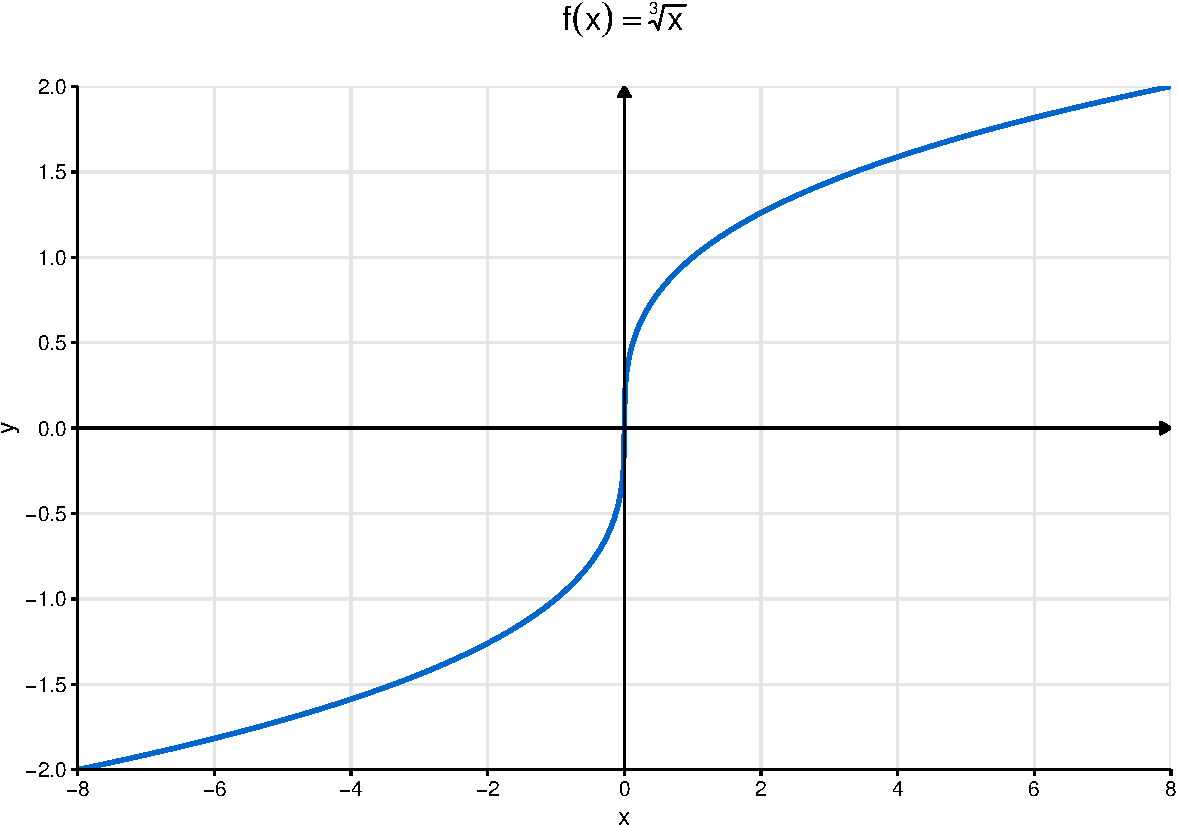
\includegraphics{exercices/Puissances/Puissances_files/figure-pdf/cubic-root-web-1.pdf}

}

\caption{Graphique de la fonction racine cubique \(f(x)=\sqrt[3]{x}\)}

\end{figure}

\end{solution}

\hypertarget{question-6-1}{%
\section{Question 6}\label{question-6-1}}

Calculer la dérivée des fonctions suivantes :

\begin{enumerate}
\item
  \(f(x) = (x^2+1)^{\frac{1}{2}}\)

  \begin{solution}

  \[f'(x) = \frac{1}{2}(x^2+1)^{-\frac{1}{2}} \cdot 2x = \frac{x}{\sqrt{x^2+1}}\]

  \end{solution}
\item
  \(g(x) = (2x+3)^{\frac{3}{2}}\)

  \begin{solution}

  \[g'(x) = \frac{3}{2}(2x+3)^{\frac{1}{2}} \cdot 2 = 3(2x+3)^{\frac{1}{2}}=3\sqrt{2x+3}\]

  \end{solution}
\item
  \(h(x) = \sqrt[3]{x^2-4}\)

  \begin{solution}

  \[h'(x) = \frac{1}{3}(x^2-4)^{-\frac{2}{3}} \cdot 2x = \frac{2x}{3(x^2-4)^{\frac{2}{3}}}=\frac{2x}{3\sqrt[3]{(x^2-4)^2}}\]

  \end{solution}
\end{enumerate}

\hypertarget{question-7-1}{%
\section{Question 7}\label{question-7-1}}

Calculer les limites suivantes :

\begin{enumerate}
\item
  \(\lim_{x \to +\infty} \dfrac{x^{\frac{5}{2}}}{x^2+1}\)

  \begin{solution}

  \[\lim_{x \to +\infty} \frac{x^{\frac{5}{2}}}{x^2+1} = \lim_{x \to +\infty} \frac{\sqrt{x}}{1+\frac{1}{x^2}} = +\infty\]

  \end{solution}
\item
  \(\lim_{x \to +\infty} \dfrac{x^{\pi}}{x^3}\)

  \begin{solution}

  \[\lim_{x \to +\infty} \frac{x^{\pi}}{x^3} = \lim_{x \to +\infty} x^{\pi-3} = +\infty \qquad(\text{car }\pi - 3>0)\]

  \end{solution}
\end{enumerate}

\hypertarget{question-8-1}{%
\section{Question 8}\label{question-8-1}}

Résoudre dans \(]0,+\infty[\) :

\begin{enumerate}
\item
  \(x^{\frac{1}{2}} = 2\)

  \begin{solution}

  \[x^{\frac{1}{2}} = 2 \iff x = 4\]

  \end{solution}
\item
  \(x^{-\frac{1}{3}} \leq 1\)

  \begin{solution}

  \[x^{-\frac{1}{3}} \leq 1 \iff x \geq 1\] car la fonction
  \(x \mapsto x^{-\frac{1}{3}}\) est décroissante sur \(]0,+\infty[\) et
  elle prend la valeur \(1\) lorsque \(x=1\).

  \end{solution}
\item
  \(x^{\frac{3}{2}} = x^{\frac{1}{2}}\)

  \begin{solution}

  \[x^{\frac{3}{2}} = x^{\frac{1}{2}} \iff x^{\frac{1}{2}}(x-1) = 0 \iff x = 0\]
  ou \(x = 1\). Dans \(]0,+\infty[\), la seule solution est \(x = 1\).

  \end{solution}
\end{enumerate}

\hypertarget{question-9-1}{%
\section{Question 9}\label{question-9-1}}

On considère la fonction \(f(x) = x^{\alpha} - x^{\beta}\) sur
\(]0,+\infty[\) avec \(\alpha > \beta > 0\).

\begin{enumerate}
\item
  Trouvez les \(x\in]0,+\infty[\) pour lesquels la dérivée de \(f\)
  s'annule.

  \begin{solution}

  \(f'(x) = \alpha x^{\alpha-1} - \beta x^{\beta-1}\)

  \(f'(x) = 0 \iff x^{\alpha-1}(\alpha - \beta x^{\beta-\alpha}) = 0\)

  \(\iff x = (\frac{\alpha}{\beta})^{\frac{1}{\alpha-\beta}}\) car
  \(x>0\).

  \end{solution}
\item
  Déterminer l'allure du graphe en utilisant le travail fait en (a).

  \begin{solution}

  La valeur de \(x\) trouvée est
  \(x_0 = (\frac{\alpha}{\beta})^{\frac{1}{\alpha-\beta}}\). On peut
  calculer la dérivée seconde et montrer qu'elle est positive à cet
  endroit. On peut aussi remarquer que la fonction s'annule seulement en
  \(x=0\) et en \(x=1\) alors qu'elle tend vers l'infini lorsque \(x\)
  devient très grand. Cela oblige \(f\) à posséder un minimum lorsque sa
  dérivée s'annule entre 0 et 1, sans quoi il y aurait forcément
  d'autres zéros de la dérivée première.

  \end{solution}
\end{enumerate}

\hypertarget{question-10-1}{%
\section{Question 10}\label{question-10-1}}

Calculer les intégrales suivantes :

\begin{enumerate}
\item
  \(\int_0^1 x^{\frac{1}{2}}dx\)

  \begin{solution}

  \[\int_0^1 x^{\frac{1}{2}}dx = \left[\frac{2}{3}x^{\frac{3}{2}}\right]_{x=0}^1 = \frac{2}{3}\]

  \end{solution}
\item
  \(\int_1^2 x^{-\frac{1}{2}}dx\)

  \begin{solution}

  \[\int_1^2 x^{-\frac{1}{2}}dx = \left[2x^{\frac{1}{2}}\right]_1^2 = 2\left(\sqrt{2}-1\right)\]

  \end{solution}
\item
  \(\int_0^4 (x^{\frac{1}{3}} + x^{\frac{2}{3}})dx\)

  \begin{solution}

  \[\int_0^4 \left(x^{\frac{1}{3}} + x^{\frac{2}{3}}\right)dx = \left[\frac{3}{4}x^{\frac{4}{3}} + \frac{3}{5}x^{\frac{5}{3}}\right]_{x=0}^4 = \frac{3}{4}4^{\frac{4}{3}} + \frac{3}{5}4^{\frac{5}{3}}=3\sqrt[3]{4}+\frac{3\sqrt[3]{4^5}}{5}\]

  \end{solution}
\end{enumerate}

\hypertarget{question-11-1}{%
\section{Question 11}\label{question-11-1}}

Montrez que pour tout \(x > 0\) et pour tout
\(\alpha,\beta \in \mathbb{R}\), on a :
\[\frac{d}{dx}(x^{\alpha}x^{\beta}) = (\alpha+\beta)x^{\alpha+\beta-1}\]

\begin{solution}

On utilise la règle du produit :

\(\frac{d}{dx}(x^{\alpha}x^{\beta}) = x^{\alpha} \cdot \frac{d}{dx}(x^{\beta}) + x^{\beta} \cdot \frac{d}{dx}(x^{\alpha})\)

\(= x^{\alpha} \cdot \beta x^{\beta-1} + x^{\beta} \cdot \alpha x^{\alpha-1}\)

\(= (\alpha+\beta)x^{\alpha+\beta-1}\)

\end{solution}

\hypertarget{lintuxe9grale-de-riemann-1}{%
\chapter{L'intégrale de Riemann}\label{lintuxe9grale-de-riemann-1}}

\hypertarget{question-1-2}{%
\chapter{Question 1}\label{question-1-2}}

Évaluez les intégrales indéfinies ci-dessous.

\begin{enumerate}
\item
  \[\int x(x^2+1)^{2007}\,\,dx\]

  \begin{solution}

  En posant \(u=x^2+1\), on obtient que \(\frac{\,du}{2}=x\,dx\). Par
  conséquent,
  \[\int x(x^2+1)^{2007}\,dx=\frac{1}{2}\int u^{2007}\,du=\frac{1}{2}\cdot\frac{u^{2008}}{2008}+C=\frac{(1+x^2)^{2008}}{4016}+C.\]

  \end{solution}
\item
  \[\int x\sqrt{x-1}\,dx\]

  \begin{solution}

  En posant \(u=x-1\), on obtient que \(\,du=\,dx\). Aussi, \(x=u+1\).
  Par conséquent, \begin{align}
  \int x\sqrt{x-1}\,dx&=\int (u+1)\sqrt{u}\,du \\
  &=\int u^{3/2}\,du+\int u^{1/2}\,du \\
  &=\frac{u^{5/2}}{5/2}+\frac{u^{3/2}}{3/2}+C \\
  &=\frac{2(x-1)^{5/2}}{5}+\frac{2(x-1)^{3/2}}{3}+C
  \end{align}

  \end{solution}
\item
  \[\int\frac{e^{2x}\,dx}{\sqrt{1+e^{2x}}}\]

  \begin{solution}

  En posant \(u=1+e^{2x}\), on obtient que
  \(\frac{\,du}{2}=e^{2x}\,dx\). Ainsi,
  \[\int\frac{e^{2x}\,dx}{\sqrt{1+e^{2x}}}=\frac{1}{2}\int\frac{\,du}{\sqrt{u}}=\frac{1}{2}\cdot\frac{u^{1/2}}{1/2}+C=\sqrt{1+e^{2x}}+C.\]

  \end{solution}
\item
  \[\int\frac{\cos(x)\sin(x)\,dx}{2+\cos(2x)}\]

  \begin{solution}

  Remarquons en premier lieu que l'intégrande est composée de fonctions
  trigonométriques d'argument différent. Pour réussir à intégrer cette
  fonction, il serait souhaitable que les fonctions trigonométriques
  présentes aient le même argument.

  \textbf{Première méthode: L'argument commun des fonctions
  trigonométrique de l'intégrande est} \(x\).

  Il nous faut ici utiliser une formule pour exprimer \(\cos(2x)\) est
  fonction de \(\sin(x)\) et de \(\cos(x)\). On sait que
  \(\cos^2(x)-\sin^2(x)=\cos(2x)\). Par conséquent,
  \[\int\frac{\cos(x)\sin(x)\,dx}{2+\cos(2x)}=\frac{\cos(x)\sin(x)\,dx}{2+\cos^2(x)-\sin^2(x)}.\]
  En posant \(u=2+\cos^2(x)-\sin^2(x)\), on trouve que
  \(\,du=-4\cos(x)\sin(x)\,dx\). Ainsi,
  \[\int\frac{\cos(x)\sin(x)\,dx}{2+\cos^2(x)-\sin^2(x)}=-\frac{1}{4}\int\frac{\,du}{u}=-\frac{1}{4}\log(2+\cos^2(x)-\sin^2(x))+C.\]

  \textbf{Deuxième méthode: l'argument commun des fonctions
  trigonométrique de l'intégrande est} \(2x\).

  On doit donc exprimer \(\cos(x)\sin(x)\) en fonction de \(\sin(2x)\)
  et de \(\cos(2x)\). Or, \(\sin(2x)=2\sin(x)\cos(x)\). Par conséquent,
  nous avons que
  \[\int\frac{\cos(x)\sin(x)\,dx}{2+\cos(2x)}=\frac{1}{2}\int\frac{\sin(2x)\,dx}{2+\cos(2x)}.\]
  En posant \(u=2+\cos(2x)\), on trouve que \(\,du=-2\sin(2x)\,dx\), et
  donc
  \[\frac{1}{2}\int\frac{\sin(2x)\,dx}{2+\cos(2x)}=-\frac{1}{4}\int\frac{\,du}{u}=-\frac{1}{4}\ln(2+\cos(2x))+C.\]

  \end{solution}
\item
  \[\int e^x\sin(x)\,dx\]

  \begin{solution}

  On pose \(u=e^x\) et \(\,dv=\sin(x)\,dx\). Ainsi, \(\,du=e^x\,dx\) et
  \(v=-\cos(x)\). Nous avons donc que \begin{align}
  \int e^x\sin(x)\,dx&=\int u\,dv \\
  &=uv-\int v\,du \\
  &=-e^x\cos(x)+\int e^x\cos(x)\,dx. \qquad(\star)
  \end{align} Il nous faut maintenant effectuer l'intégrale de la
  fonction \(e^x\cos(x)\). Encore une fois, on procède en utilisant la
  méthode d'intégration par parties. Posons \(r=e^x\) et
  \(\,ds=\cos(x)\,dx\). On obtient que \(\,dr=e^x\,dx\) et
  \(s=\sin(x)\). On a ainsi que \begin{align}
  \int e^x\cos(x)\,dx&=\int r\,ds \\
  &=rs-\int s\,dr \\
  &=e^x\sin(x)-\int e^x\sin(x)\,dx. \qquad(\star\star)
  \end{align} Nous voyons apparaître à nouveau l'intégrale qui est en
  fait l'inconnu de notre problème de départ. On pourrait penser que
  tout ce que nous avons fait dans ce problème jusqu'à présent est
  tourner en rond. Cependant, il n'en est rien de cela puisqu'en
  utilisant les équations \((\star)\) et \((\star\star)\), on obtient
  que \begin{align}
  \int e^x\sin(x)\,dx&=-e^x\cos(x)+\int e^x\cos(x)\,dx & \qquad(\text{d'après}(\star)) \\
  &=-e^x\cos(x)+e^x\sin(x)-\int e^x\sin(x)\,dx. & \qquad(\text{d'après}(\star\star))
  \end{align} Ainsi, \(2\int e^x\sin(x)\,dx=-e^x\cos(x)+e^x\sin(x)\),
  d'où
  \[\int e^x\sin(x)\,dx=\frac{e^x}{2}\left(\sin(x)-\cos(x)\right)+C.\]

  \end{solution}
\item
  \[\int\arctan(x)\,dx\]

  \begin{solution}

  On pose \(u=\arctan(x)\) et \(\,dv=\,dx\). Ainsi,
  \(\,du=\frac{\,dx}{1+x^2}\) et \(v=x\). Nous avons donc que
  \begin{align}
  \int\arctan(x)\,dx&=\int u\,dv \\
  &=uv-\int v\,du \\
  &=x\arctan(x)-\int \frac{x\,dx}{1+x^2}.
  \end{align} En posant \(r=1+x^2\), on trouve que
  \(\frac{\,dr}{2}=x\,dx\), d'où
  \[\int\frac{x\,dx}{1+x^2}=\frac{1}{2}\int\frac{\,dr}{r}=\frac{1}{2}\log(1+x^2)+C.\]
  Ainsi,
  \[\int\arctan(x)\,dx=x\arctan(x)-\frac{1}{2}\log(1+x^2)+C=x\arctan(x)-\log\left(\sqrt{1+x^2}\right)+C.\]

  \end{solution}
\item
  \[\int\sin(\log x)\,dx\]

  \begin{solution}

  On pose \(u=\sin(\log x)\) et \(\,dv=\,dx\). Ainsi,
  \(\,du=\frac{\cos(\log x)\,dx}{x}\) et \(v=x\). Nous avons donc que
  \begin{align}
  \int\sin(\log x)\,dx&=\int u\,dv \\
  &=uv-\int v\,du \\
  &=x\sin(\log x)-\int \cos(\log x)\,dx. \qquad(\star)
  \end{align} Il nous faut maintenant effectuer l'intégrale de la
  fonction \(\cos(\log x)\). On procède encore en utilisant la méthode
  d'intégration par parties. Posons \(r=\cos(\log x)\) et \(\,ds=\,dx\).
  On obtient que \(\,dr=-\frac{\sin(\log x)}{x}\,dx\) et \(s=x\). On a
  ainsi que \begin{align}
  \int \cos(\log x)\,dx&=\int r\,ds \\
  &=rs-\int s\,dr \\
  &=x\cos(\log x)+\int \sin(\log x)\,dx. \qquad(\star\star)
  \end{align} Les équations \((\star)\) et \((\star\star)\) entraînent
  que
  \[\int\sin(\log x)\,dx=x\sin(\log x)-x\cos(\log x )-\int \sin(\log x)\,dx,\]
  d'où
  \[\int\sin(\log x)\,dx=\frac{x}{2}\left(\sin(\log x)-\cos(\log x)\right)+C.\]

  \end{solution}
\item
  \[\int\frac{\,dx}{\sqrt{1-x^2}}\]

  \begin{solution}

  On pose \(x=\cos\theta\), d'où \(\,dx=-\sin\theta \,d\theta\). Ainsi,
  \begin{align}
  \int\frac{\,dx}{\sqrt{1-x^2}}&=-\int\frac{\sin\theta \,d\theta}{\sqrt{1-\cos^2\theta}} \\
  &=-\int\frac{\sin\theta \,d\theta}{\sqrt{\sin^2\theta}} \\
  &=-\int \,d\theta \\
  &=-\theta +C \\
  &=-\arccos x +C
  \end{align}

  \end{solution}
\item
  \[\int\frac{\,dx}{x^3-x^2+x-1}\]

  \begin{solution}

  On observe que le dénominateur s'annule lorsque \(x=1\). Ainsi,
  \(x-1\) est un de ses facteurs. En divisant \(x^3-x^2+x-1\) par
  \(x-1\), on obtient \(1+x^2\). Il existe donc des constantes \(A,B\)
  et \(C\) telles que
  \[\frac{1}{x^3-x^2+x-1}=\frac{A}{x-1}+\frac{Bx+C}{1+x^2}.\] On trouve
  que \(A=1/2\) et \(B=C=-1/2\). Comme
  \(\int\frac{1/2\,dx}{x-1}=\frac{1}{2}\ln (x-1)+C_1\) et
  \(\int-\frac{1}{2}\frac{(x+1)\,dx}{1+x^2}=-\frac{1}{4}\ln (x^2+1)-\frac{1}{2}\arctan (x)+C_2\),
  il suit que
  \[\int\frac{\,dx}{x^3-x^2+x-1}=\frac{1}{2}\ln (x-1)-\frac{1}{4}\ln (x^2+1)-\frac{1}{2}\arctan (x)+C.\]

  \end{solution}
\item
  \[\int\frac{\,dx}{\sqrt{9+4x^2}}\]

  \begin{solution}

  \begin{align}
  \int\frac{\,dx}{\sqrt{9+4x^2}}&=\frac{1}{3}\int\frac{\,dx}{\frac{1}{3}\sqrt{9+4x^2}} \\
  &=\frac{1}{3}\int\frac{\,dx}{\sqrt{1+\frac{4x^2}{9}}} \\
  &=\frac{1}{3}\int\frac{\,dx}{\sqrt{1+\left(\frac{2x}{3}\right)^2}}
  \end{align} Posons \(u=\frac{2x}{3}\). Ainsi,
  \(\frac{3}{2}\,du=\,dx\), d'où
  \[\int\frac{\,dx}{\sqrt{9+4x^2}}=\frac{1}{3}\int\frac{\,dx}{\sqrt{1+\left(\frac{2x}{3}\right)^2}}=\frac{1}{2}\int\frac{\,du}{\sqrt{1+u^2}}.\]
  On effectue maintenant le changement de variable \(u=\tan\theta\).
  Nous avons donc que \(\,du=\sec^2\theta \,d\theta\), ce qui nous
  permet d'écrire que \begin{align}
  \frac{1}{2}\int\frac{\,du}{\sqrt{1+u^2}}&=\frac{1}{2}\int\frac{\sec^2\theta \,d\theta}{\sqrt{1+\tan^2\theta}} \\
  &=\frac{1}{2}\int\frac{\sec^2\theta \,d\theta}{\sqrt{\sec^2\theta}} \\
  &=\frac{1}{2}\int\sec\theta \,d\theta \\
  &=\frac{1}{2}\log|\sec\theta+\tan\theta|+C \\
  &=\frac{1}{2}\log|\sqrt{1+u^2}+u|+C \\
  &=\frac{1}{2}\log\left|\sqrt{1+\left(\frac{2x}{3}\right)^2}+\frac{2x}{3}\right|+C \\
  &=\frac{1}{2}\log\left|\frac{1}{3}\sqrt{9+4x^2}+\frac{2x}{3}\right|+C \\
  &=\frac{1}{2}\log\left|\frac{1}{3}\left(\sqrt{9+4x^2}+2x\right)\right|+C \\
  &=\frac{1}{2}\log\frac{1}{3}+\frac{1}{2}\log\left|\sqrt{9+4x^2}+2x\right|+C \\
  &=\frac{1}{2}\log\left|\sqrt{9+4x^2}+2x\right|+D
  \end{align}

  \end{solution}
\item
  \[\int\frac{\,dx}{\sqrt{x^2-2x+5}}\]

  \begin{solution}

  En complétant le carré, on obtient que
  \[\int\frac{\,dx}{\sqrt{x^2-2x+5}}=\int\frac{\,dx}{\sqrt{(x-1)^2+4}}.\]
  En posant \(u=x-1\), on trouve que \(\,dx=\,du\), ce qui permet
  d'écrire \begin{align}
  \int\frac{\,dx}{\sqrt{(x-1)^2+4}}&=\int\frac{\,du}{\sqrt{u^2+4}} \\
  &=\frac{1}{2}\int\frac{\,du}{\frac{1}{2}\sqrt{u^2+4}} \\
  &=\frac{1}{2}\int\frac{\,du}{\sqrt{\left(\frac{u}{2}\right)^2+1}} \\
  &=\int\frac{\,dv}{\sqrt{v^2+1}}. \qquad\text{(en posant $v=u/2$)}
  \end{align} Au numéro précédent, nous avons montré que
  \[\int\frac{\,dv}{\sqrt{v^2+1}}=\log\left|\sqrt{1+v^2}+v\right|+C.\]
  Par conséquent, \begin{align}
  \int\frac{\,dx}{\sqrt{x^2-2x+5}}&=\log\left|\sqrt{1+v^2}+v\right|+C \\
  &=\log\left|\sqrt{1+u^2/4}+u/2\right|+C \\
  &=\log\left|\frac{1}{2}\sqrt{4+u^2}+u/2\right|+C \\
  &=\log\left|\frac{\sqrt{4+u^2}+u}{2}\right|+C \\
  &=\log\left|\sqrt{4+u^2}+u\right|+D \\
  &=\log\left|\sqrt{4+(x-1)^2}+x-1\right|+D
  \end{align}

  \end{solution}
\item
  \[\int\frac{e^{2x}\,dx}{1+e^{4x}}\]

  \begin{solution}

  Posons \(u=e^{2x}\). Ainsi, \(\frac{\,du}{2}=e^{2x}\,dx\) et
  \(u^2=e^{4x}\). On peut donc écrire \begin{align}
  \int\frac{e^{2x}\,dx}{1+e^{4x}}&=\frac{1}{2}\int\frac{\,du}{1+u^2} \\
  &=\arctan(u)+C \\
  &=\frac{\arctan(e^{2x})}{2}+C
  \end{align}

  \end{solution}
\end{enumerate}

\hypertarget{question-2-2}{%
\section{Question 2}\label{question-2-2}}

Évaluez les intégrales définies ci-dessous.

\begin{enumerate}
\item
  \[\int_{1}^{\infty}\frac{\,dx}{x}\]

  \begin{solution}

  Nous avons que
  \[\int_{1}^{\infty}\frac{\,dx}{x}=\lim_{b\rightarrow\infty}\int_{1}^{b}\frac{\,dx}{x}=\lim_{b\rightarrow\infty}\left(\log b-\log 1\right)=\infty.\]

  \end{solution}
\item
  \[\int_{-\pi}^{\pi}\sin^2(x)\,dx\]

  \begin{solution}

  Nous avons que \(\sin^2(x)=\frac{1-\cos(2x)}{2}\). Ainsi,
  \begin{align}
  \int_{-\pi}^{\pi}\sin^2(x)\,dx&=\int_{-\pi}^{\pi}\frac{1-\cos(2x)}{2}\,dx \\
  &=\frac{1}{2}\int_{-\pi}^{\pi}\,dx-\frac{1}{2}\int_{-\pi}^{\pi}\cos(2x)\,dx \\
  &=\left. \frac{x}{2}\right|_{x=-\pi}^{\pi}-\left. \frac{1}{4}\sin(2x)\right|_{x=-\pi}^{\pi} \\
  &=\pi
  \end{align}

  \end{solution}
\item
  \[\int_{0}^{\pi/4}\tan\left(\frac{\theta}{2}\right)\,dx\]

  \begin{solution}

  Posons \(u=\theta/2\). Ainsi, \(2\,du=\,d\theta\). Nous avons donc que
  \begin{align}
  \int_{0}^{\pi/4}\tan\left(\frac{\theta}{2}\right)\,d\theta&=2\int_{\theta=0}^{\theta=\pi/4}\tan(u)\,du \\
  &=\left. 2\log|\sec u|\right|_{\theta=0}^{\theta=\pi/4} \\
  &=\left. 2\log\left|\sec \theta/2\right|\right|_{0}^{\pi/4} \\
  &=2\left(\frac{1}{\cos \frac{\pi}{8}}-\frac{1}{\cos 0}\right) \\
  &=2\left(\frac{1}{\sqrt{2+\sqrt{2}}}-1\right) \\
  &=\frac{2\left(\sqrt{2+\sqrt{2}}-2-\sqrt{2}\right)}{2+\sqrt{2}}
  \end{align} Pour obtenir que \(\cos(\pi/8)=\sqrt{2+\sqrt{2}}\), nous
  avons utilisé l'identité \(\cos^2(x)=\frac{1+\cos(2x)}{2}\) en
  observant que \(\cos(\pi/4)=\sqrt{2}/2\) et en posant \(x=\pi/4\).

  \end{solution}
\end{enumerate}

\hypertarget{question-3-2}{%
\section{Question 3}\label{question-3-2}}

Représentez la région bornée délimitée par les courbes \(y=x\sin x\),
\(y=-x\), \(x=0\) et \(x=\tfrac{3\pi}{2}\) dans le plan \(Oxy\).
Déterminez ensuite son aire.

\begin{solution}

Nous allons représenter la région bornée délimitée par les courbes
suivantes : 1. \(y = x\sin(x)\) 2. \(y = -x\) 3. \(x = 0\) 4.
\(x = \frac{3\pi}{2}\)

\begin{Shaded}
\begin{Highlighting}[]
\ImportTok{import}\NormalTok{ numpy }\ImportTok{as}\NormalTok{ np}
\ImportTok{import}\NormalTok{ matplotlib.pyplot }\ImportTok{as}\NormalTok{ plt}
\CommentTok{\# Création des points pour les courbes}
\NormalTok{x }\OperatorTok{=}\NormalTok{ np.linspace(}\DecValTok{0}\NormalTok{, }\DecValTok{3}\OperatorTok{*}\NormalTok{np.pi}\OperatorTok{/}\DecValTok{2}\NormalTok{, }\DecValTok{1000}\NormalTok{)}
\NormalTok{y1 }\OperatorTok{=}\NormalTok{ x }\OperatorTok{*}\NormalTok{ np.sin(x)  }\CommentTok{\# Courbe y = x*sin(x)}
\NormalTok{y2 }\OperatorTok{=} \OperatorTok{{-}}\NormalTok{x             }\CommentTok{\# Droite y = {-}x}
\CommentTok{\# Création de la figure}
\NormalTok{plt.figure(figsize}\OperatorTok{=}\NormalTok{(}\FloatTok{7.5}\NormalTok{, }\DecValTok{8}\NormalTok{))}
\CommentTok{\# Tracer les courbes}
\NormalTok{plt.plot(x, y1, }\StringTok{\textquotesingle{}b{-}\textquotesingle{}}\NormalTok{, label}\OperatorTok{=}\StringTok{\textquotesingle{}y = x·sin(x)\textquotesingle{}}\NormalTok{)}
\NormalTok{plt.plot(x, y2, }\StringTok{\textquotesingle{}r{-}\textquotesingle{}}\NormalTok{, label}\OperatorTok{=}\StringTok{\textquotesingle{}y = {-}x\textquotesingle{}}\NormalTok{)  }\CommentTok{\# Changé ici de \textquotesingle{}b{-}\textquotesingle{} à \textquotesingle{}r{-}\textquotesingle{}}
\CommentTok{\# Remplir la région entre les courbes}
\NormalTok{plt.fill\_between(x, y1, y2, color}\OperatorTok{=}\StringTok{\textquotesingle{}darkblue\textquotesingle{}}\NormalTok{, alpha}\OperatorTok{=}\FloatTok{0.3}\NormalTok{)}
\NormalTok{plt.axvline(x}\OperatorTok{=}\DecValTok{3}\OperatorTok{*}\NormalTok{np.pi}\OperatorTok{/}\DecValTok{2}\NormalTok{, color}\OperatorTok{=}\StringTok{\textquotesingle{}k\textquotesingle{}}\NormalTok{, linestyle}\OperatorTok{=}\StringTok{\textquotesingle{}{-}{-}\textquotesingle{}}\NormalTok{, label}\OperatorTok{=}\StringTok{\textquotesingle{}x = 3π/2\textquotesingle{}}\NormalTok{)}
\CommentTok{\# Paramètres des axes}
\NormalTok{plt.axhline(y}\OperatorTok{=}\DecValTok{0}\NormalTok{, color}\OperatorTok{=}\StringTok{\textquotesingle{}k\textquotesingle{}}\NormalTok{, linestyle}\OperatorTok{=}\StringTok{\textquotesingle{}{-}\textquotesingle{}}\NormalTok{, alpha}\OperatorTok{=}\FloatTok{0.3}\NormalTok{)}
\NormalTok{plt.axvline(x}\OperatorTok{=}\DecValTok{0}\NormalTok{, color}\OperatorTok{=}\StringTok{\textquotesingle{}k\textquotesingle{}}\NormalTok{, linestyle}\OperatorTok{=}\StringTok{\textquotesingle{}{-}\textquotesingle{}}\NormalTok{, alpha}\OperatorTok{=}\FloatTok{0.3}\NormalTok{)}
\CommentTok{\# Étiquettes des axes}
\NormalTok{plt.xlabel(}\StringTok{\textquotesingle{}x\textquotesingle{}}\NormalTok{)}
\NormalTok{plt.ylabel(}\StringTok{\textquotesingle{}y\textquotesingle{}}\NormalTok{)}
\CommentTok{\# Limites des axes}
\NormalTok{plt.xlim(}\OperatorTok{{-}}\FloatTok{0.1}\NormalTok{, }\DecValTok{5}\NormalTok{)}
\NormalTok{plt.ylim(}\OperatorTok{{-}}\DecValTok{5}\NormalTok{, }\DecValTok{5}\NormalTok{)}
\CommentTok{\# Ajouter les ticks spéciaux pour}
\NormalTok{ticks }\OperatorTok{=}\NormalTok{ [}\DecValTok{0}\NormalTok{, np.pi}\OperatorTok{/}\DecValTok{2}\NormalTok{, np.pi, }\DecValTok{3}\OperatorTok{*}\NormalTok{np.pi}\OperatorTok{/}\DecValTok{2}\NormalTok{]}
\NormalTok{labels }\OperatorTok{=}\NormalTok{ [}\StringTok{\textquotesingle{}0\textquotesingle{}}\NormalTok{, }\StringTok{\textquotesingle{}π/2\textquotesingle{}}\NormalTok{, }\StringTok{\textquotesingle{}π\textquotesingle{}}\NormalTok{, }\StringTok{\textquotesingle{}3π/2\textquotesingle{}}\NormalTok{]}
\NormalTok{plt.xticks(ticks, labels)}
\CommentTok{\# Ajouter une grille}
\NormalTok{plt.grid(}\VariableTok{True}\NormalTok{, alpha}\OperatorTok{=}\FloatTok{0.3}\NormalTok{)}
\CommentTok{\# Ajouter une légende}
\NormalTok{plt.legend()}
\CommentTok{\# Ajuster la mise en page}
\NormalTok{plt.tight\_layout()}
\CommentTok{\# Afficher le graphique}
\NormalTok{plt.show()}
\end{Highlighting}
\end{Shaded}

\begin{figure}[H]

{\centering 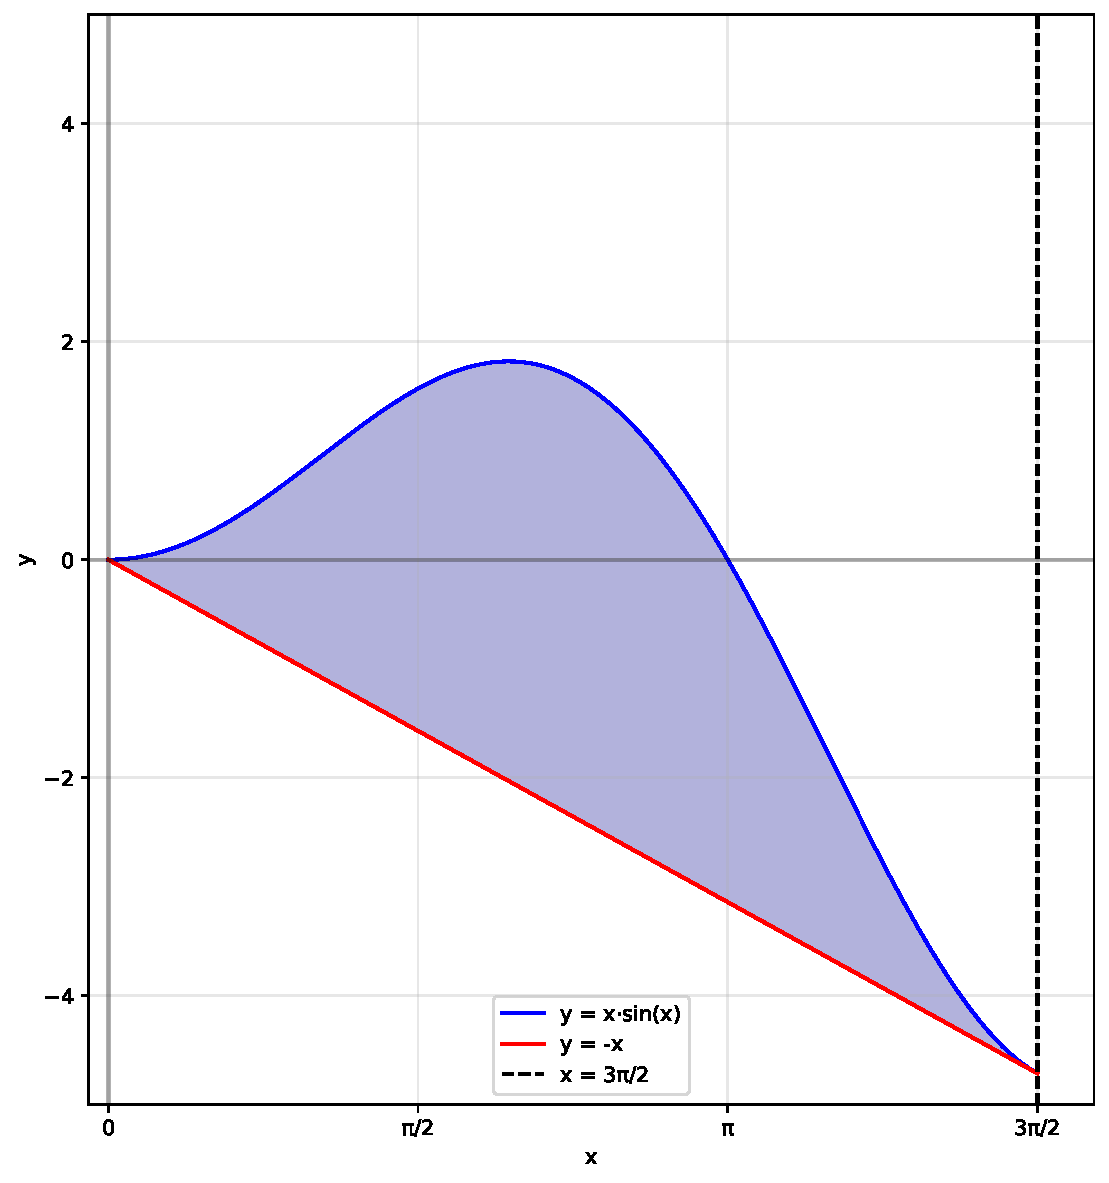
\includegraphics{exercices/IntegraleRiemann/IntegraleRiemann_files/figure-pdf/fig-region-output-1.pdf}

}

\caption{\label{fig-region}Région bornée par les courbes}

\end{figure}

L'aire de la région considérée correspond à l'intégrale
\(\int_{0}^{\frac{3\pi}{2}}(x\sin(x)-(-x))\,dx\). D'abord, en intégrant
par parties, on trouve que la fonction \(-x\cos(x)+\sin(x)\) est une
primitive de la fonction \(x\sin(x)\). Ainsi, \begin{align}
\int_{0}^{\frac{3\pi}{2}}(x\sin(x)-(-x))\,dx&=\int_{0}^{\frac{3\pi}{2}}x\sin(x)\,dx+\int_{0}^{\frac{3\pi}{2}}x\,dx \\
&=\left(-x\cos(x)+\sin(x)\right)\Big|_{0}^{\frac{3\pi}{2}}+\frac{x^2}{2}\Big|_{0}^{\frac{3\pi}{2}} \\
&=\frac{9\pi^2-8}{8}
\end{align}

\end{solution}

\hypertarget{question-4-2}{%
\section{Question 4}\label{question-4-2}}

En utilisant la méthode de Riemann, montrez que
\(\int_0^1x^2\,dx=\frac{1}{3}\).

\begin{solution}

On divise l'intervalle \([0,1]\) en \(n\) intervalles de longueur
\(1/n\). Soit \(A_n\) l'aire de la région occupée par les \(n\)
rectangles inscrits sous la parabole. Posons \(f(x)=x^2\). Ainsi,
\begin{align}
A_n&=\frac{1}{n}f(0)+\frac{1}{n}f\left(0+\frac{1}{n}\right)+\frac{1}{n}f\left(0+\frac{2}{n}\right)+\ldots+\frac{1}{n}f\left(0+\frac{n-1}{n}\right) \\
&=\frac{1}{n}\sum_{k=0}^{n-1}f\left(\frac{k}{n}\right) \\
&=\frac{1}{n}\sum_{k=0}^{n-1}\frac{k^2}{n^2} \\
&=\frac{1}{n^3}\sum_{k=0}^{n-1}k^2 \\
&=\frac{1}{n^3}\cdot\frac{n(n-1)(2(n-1)+1)}{6} \\
&=\frac{(n-1)(2n-1)}{6n^2}
\end{align} Au passage, nous avons utilisé la formule
\(\sum_{k=1}^nk^2=\frac{n(n+1)(2n+1)}{6}\). Ainsi, \begin{align}
\int_{0}^1 x^2\,dx&=\lim_{n\rightarrow\infty}A_n=\lim_{n\rightarrow\infty}\frac{(n-1)(2n-1)}{6n^2} \\
&=\lim_{n\rightarrow\infty}\frac{2n^2-3n+1}{6n^2} \\
&=1/3.
\end{align}

\end{solution}

\hypertarget{question-5-2}{%
\section{Question 5}\label{question-5-2}}

Soit \(a\in\mathbb{R}\) et soit \(f\) une fonction continue et impaire
sur l'intervalle \([-a,a]\). Montrez que \(\int_{-a}^{a}f(x)\,dx=0\).

\begin{solution}

Géométriquement, le fait que la fonction soit impaire entraîne que l'axe
des \(x\) partage la région entre le graphe de la fonction et l'axe des
\(x\) en deux régions dont l'aire géométrique est la même. La région
sous l'axe des \(x\) possède une aire algébrique négative, et celle
au-dessus de l'axe des \(x\) possède une aire algébrique positive. Donc
en choisissant un intervalle qui possède son point milieu en 0, on a
nécessairement que la somme de l'aire (algébrique) de la région
considérée est nulle. \begin{align}
\int_{-a}^{0}f(x)\,dx&=\int_{-a}^{0}-f(-x)\,dx & \qquad\text{(car $f(-x)=-f(x)$ si $f$ est impaire)} \\
&=-\int_{x=-a}^{x=0}f(-x)\,dx \\
&=\int_{x=-a}^{x=0}f(u)\,du & \qquad \text{(en posant $u=-x$)} \\
&=\int_{u=a}^{u=0}f(u)\,du \\
&=-\int_{u=0}^{u=a}f(u)\,du & \qquad \text{(propriété de l'intégrale)} \\
&=-\int_{0}^{a}f(u)\,du.
\end{align}

\end{solution}

\hypertarget{question-6-2}{%
\section{Question 6}\label{question-6-2}}

Évaluez l'intégrale définie
\[\int_{-\pi}^{\pi}x^{2017}\sin\left(\frac{1}{x^2+1}\right)\,dx.\]

\begin{solution}

La fonction est impaire et l'intervalle d'intégration est symétrique par
rapport à \(0\), donc l'intégrale vaut \(0\).

\end{solution}

\hypertarget{les-fonctions-hyperboliques-1}{%
\chapter{Les fonctions
hyperboliques}\label{les-fonctions-hyperboliques-1}}

\hypertarget{question-1-3}{%
\section{Question 1}\label{question-1-3}}

\begin{enumerate}
\def\labelenumi{\arabic{enumi}.}
\item
  La fonction \(\tanh x\) est définie par :
  \[\tanh x = \frac{\sinh x}{\cosh x}.\] Effectuez l'analyse de cette
  fonction afin de pouvoir esquisser son graphique.

  \begin{solution}

\begin{Shaded}
\begin{Highlighting}[]
\ImportTok{import}\NormalTok{ numpy }\ImportTok{as}\NormalTok{ np}
\ImportTok{import}\NormalTok{ matplotlib.pyplot }\ImportTok{as}\NormalTok{ plt}

\CommentTok{\# Création des données}
\NormalTok{x }\OperatorTok{=}\NormalTok{ np.linspace(}\OperatorTok{{-}}\DecValTok{4}\NormalTok{, }\DecValTok{4}\NormalTok{, }\DecValTok{1000}\NormalTok{)  }\CommentTok{\# Intervalle de {-}4 à 4}
\NormalTok{y }\OperatorTok{=}\NormalTok{ np.tanh(x)}

\CommentTok{\# Création de la figure}
\NormalTok{plt.figure(figsize}\OperatorTok{=}\NormalTok{(}\FloatTok{7.5}\NormalTok{, }\DecValTok{6}\NormalTok{))}

\CommentTok{\# Tracé de la fonction}
\NormalTok{plt.plot(x, y, }\StringTok{\textquotesingle{}b{-}\textquotesingle{}}\NormalTok{, label}\OperatorTok{=}\StringTok{\textquotesingle{}tanh(x)\textquotesingle{}}\NormalTok{)}

\CommentTok{\# Ajout des asymptotes horizontales}
\NormalTok{plt.axhline(y}\OperatorTok{=}\DecValTok{1}\NormalTok{, color}\OperatorTok{=}\StringTok{\textquotesingle{}r\textquotesingle{}}\NormalTok{, linestyle}\OperatorTok{=}\StringTok{\textquotesingle{}{-}{-}\textquotesingle{}}\NormalTok{, alpha}\OperatorTok{=}\FloatTok{0.5}\NormalTok{, label}\OperatorTok{=}\StringTok{\textquotesingle{}y = ±1\textquotesingle{}}\NormalTok{)}
\NormalTok{plt.axhline(y}\OperatorTok{={-}}\DecValTok{1}\NormalTok{, color}\OperatorTok{=}\StringTok{\textquotesingle{}r\textquotesingle{}}\NormalTok{, linestyle}\OperatorTok{=}\StringTok{\textquotesingle{}{-}{-}\textquotesingle{}}\NormalTok{, alpha}\OperatorTok{=}\FloatTok{0.5}\NormalTok{)}

\CommentTok{\# Ajout des axes}
\NormalTok{plt.axhline(y}\OperatorTok{=}\DecValTok{0}\NormalTok{, color}\OperatorTok{=}\StringTok{\textquotesingle{}k\textquotesingle{}}\NormalTok{, linestyle}\OperatorTok{=}\StringTok{\textquotesingle{}{-}\textquotesingle{}}\NormalTok{, alpha}\OperatorTok{=}\FloatTok{0.3}\NormalTok{)}
\NormalTok{plt.axvline(x}\OperatorTok{=}\DecValTok{0}\NormalTok{, color}\OperatorTok{=}\StringTok{\textquotesingle{}k\textquotesingle{}}\NormalTok{, linestyle}\OperatorTok{=}\StringTok{\textquotesingle{}{-}\textquotesingle{}}\NormalTok{, alpha}\OperatorTok{=}\FloatTok{0.3}\NormalTok{)}

\CommentTok{\# Configuration du graphique}
\NormalTok{plt.grid(}\VariableTok{True}\NormalTok{, alpha}\OperatorTok{=}\FloatTok{0.3}\NormalTok{)}
\NormalTok{plt.title(}\StringTok{\textquotesingle{}Fonction tanh(x)\textquotesingle{}}\NormalTok{)}
\NormalTok{plt.xlabel(}\StringTok{\textquotesingle{}x\textquotesingle{}}\NormalTok{)}
\NormalTok{plt.ylabel(}\StringTok{\textquotesingle{}y\textquotesingle{}}\NormalTok{)}
\NormalTok{plt.legend()}

\CommentTok{\# Ajustement des limites}
\NormalTok{plt.ylim(}\OperatorTok{{-}}\FloatTok{1.5}\NormalTok{, }\FloatTok{1.5}\NormalTok{)}

\NormalTok{plt.show()}
\end{Highlighting}
\end{Shaded}

  \begin{figure}[H]

  {\centering 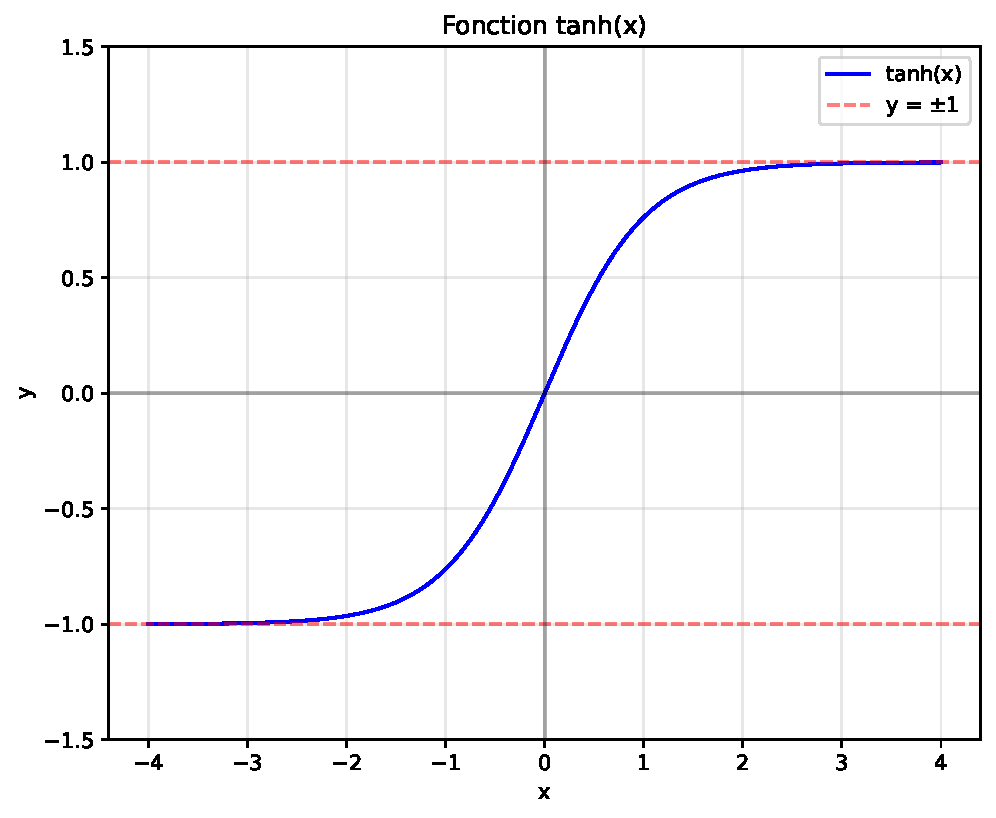
\includegraphics{exercices/FonctionsHyp/FonctionsHyp_files/figure-pdf/cell-2-output-1.pdf}

  }

  \end{figure}

  \end{solution}
\item
  Montrez que la fonction réciproque de \(\tanh x\), notée
  \(\text{arctanh}\,x\), peut s'exprimer par
  \[\text{arctanh}\,x = \ln \sqrt{\frac{1+x}{1-x}}.\]

  \begin{solution}

  Montrons que \(\text{arctanh}\,x = \ln \sqrt{\frac{1+x}{1-x}}\).
  Posons \(y = \text{arctanh}\,x\). Par définition, cela signifie que
  \(x = \tanh y\). La fonction tanh est définie par :
  \[\tanh y = \frac{\sinh y}{\cosh y} = \frac{e^y - e^{-y}}{e^y + e^{-y}}.\]
  Donc nous avons que \(x = \dfrac{e^y - e^{-y}}{e^y + e^{-y}}\).
  Multiplions les deux membres par \((e^y + e^{-y})\) :
  \[x(e^y + e^{-y}) = e^y - e^{-y}.\] Développons :
  \[xe^y + xe^{-y} = e^y - e^{-y}.\] Regroupons les termes en \(e^y\) et
  \(e^{-y}\) : \[e^y(x-1) = e^{-y}(x+1).\] Donc :
  \[\frac{e^y}{e^{-y}} = \frac{x+1}{1-x}.\qquad(x\neq 1)\] Simplifions :
  \[e^{2y} = \frac{1+x}{1-x}.\] Prenons le logarithme naturel des deux
  côtés : \[2y = \ln\left(\frac{1+x}{1-x}\right).\] Donc :
  \[y = \frac{1}{2}\ln\left(\frac{1+x}{1-x}\right) = \ln\sqrt{\frac{1+x}{1-x}}.\]
  Puisque \(y = \text{arctanh}\,x\), nous avons bien
  \[\text{arctanh}\,x = \ln\sqrt{\frac{1+x}{1-x}}.\]

  \end{solution}
\item
  Esquissez le graphique de \(\text{arctanh}\,x\).

  \begin{solution}

\begin{Shaded}
\begin{Highlighting}[]
\ImportTok{import}\NormalTok{ numpy }\ImportTok{as}\NormalTok{ np}
\ImportTok{import}\NormalTok{ matplotlib.pyplot }\ImportTok{as}\NormalTok{ plt}
\CommentTok{\# Création des données}
\NormalTok{x }\OperatorTok{=}\NormalTok{ np.linspace(}\OperatorTok{{-}}\FloatTok{0.99}\NormalTok{, }\FloatTok{0.99}\NormalTok{, }\DecValTok{1000}\NormalTok{)  }\CommentTok{\# On évite {-}1 et 1 car arctanh non défini}
\NormalTok{y }\OperatorTok{=}\NormalTok{ np.arctanh(x)}
\CommentTok{\# Création de la figure}
\NormalTok{plt.figure(figsize}\OperatorTok{=}\NormalTok{(}\DecValTok{8}\NormalTok{, }\DecValTok{6}\NormalTok{))}
\CommentTok{\# Tracé de la fonction}
\NormalTok{plt.plot(x, y, }\StringTok{\textquotesingle{}b{-}\textquotesingle{}}\NormalTok{, label}\OperatorTok{=}\StringTok{\textquotesingle{}arctanh(x)\textquotesingle{}}\NormalTok{)}
\CommentTok{\# Ajout des axes}
\NormalTok{plt.axhline(y}\OperatorTok{=}\DecValTok{0}\NormalTok{, color}\OperatorTok{=}\StringTok{\textquotesingle{}k\textquotesingle{}}\NormalTok{, linestyle}\OperatorTok{=}\StringTok{\textquotesingle{}{-}\textquotesingle{}}\NormalTok{, alpha}\OperatorTok{=}\FloatTok{0.3}\NormalTok{)}
\NormalTok{plt.axvline(x}\OperatorTok{=}\DecValTok{0}\NormalTok{, color}\OperatorTok{=}\StringTok{\textquotesingle{}k\textquotesingle{}}\NormalTok{, linestyle}\OperatorTok{=}\StringTok{\textquotesingle{}{-}\textquotesingle{}}\NormalTok{, alpha}\OperatorTok{=}\FloatTok{0.3}\NormalTok{)}
\CommentTok{\# Ajout des asymptotes verticales}
\NormalTok{plt.axvline(x}\OperatorTok{=}\DecValTok{1}\NormalTok{, color}\OperatorTok{=}\StringTok{\textquotesingle{}r\textquotesingle{}}\NormalTok{, linestyle}\OperatorTok{=}\StringTok{\textquotesingle{}{-}{-}\textquotesingle{}}\NormalTok{, alpha}\OperatorTok{=}\FloatTok{0.5}\NormalTok{, label}\OperatorTok{=}\StringTok{\textquotesingle{}x = ±1\textquotesingle{}}\NormalTok{)}
\NormalTok{plt.axvline(x}\OperatorTok{={-}}\DecValTok{1}\NormalTok{, color}\OperatorTok{=}\StringTok{\textquotesingle{}r\textquotesingle{}}\NormalTok{, linestyle}\OperatorTok{=}\StringTok{\textquotesingle{}{-}{-}\textquotesingle{}}\NormalTok{, alpha}\OperatorTok{=}\FloatTok{0.5}\NormalTok{)}
\CommentTok{\# Configuration du graphique}
\NormalTok{plt.grid(}\VariableTok{True}\NormalTok{, alpha}\OperatorTok{=}\FloatTok{0.3}\NormalTok{)}
\NormalTok{plt.title(}\StringTok{\textquotesingle{}Fonction arctanh(x)\textquotesingle{}}\NormalTok{)}
\NormalTok{plt.xlabel(}\StringTok{\textquotesingle{}x\textquotesingle{}}\NormalTok{)}
\NormalTok{plt.ylabel(}\StringTok{\textquotesingle{}y\textquotesingle{}}\NormalTok{)}
\NormalTok{plt.legend()}
\CommentTok{\# Ajustement des limites pour mieux voir les asymptotes}
\NormalTok{plt.ylim(}\OperatorTok{{-}}\DecValTok{4}\NormalTok{, }\DecValTok{4}\NormalTok{)}
\NormalTok{plt.xlim(}\OperatorTok{{-}}\FloatTok{1.1}\NormalTok{, }\FloatTok{1.1}\NormalTok{)}
\NormalTok{plt.show()}
\end{Highlighting}
\end{Shaded}

  \begin{figure}[H]

  {\centering 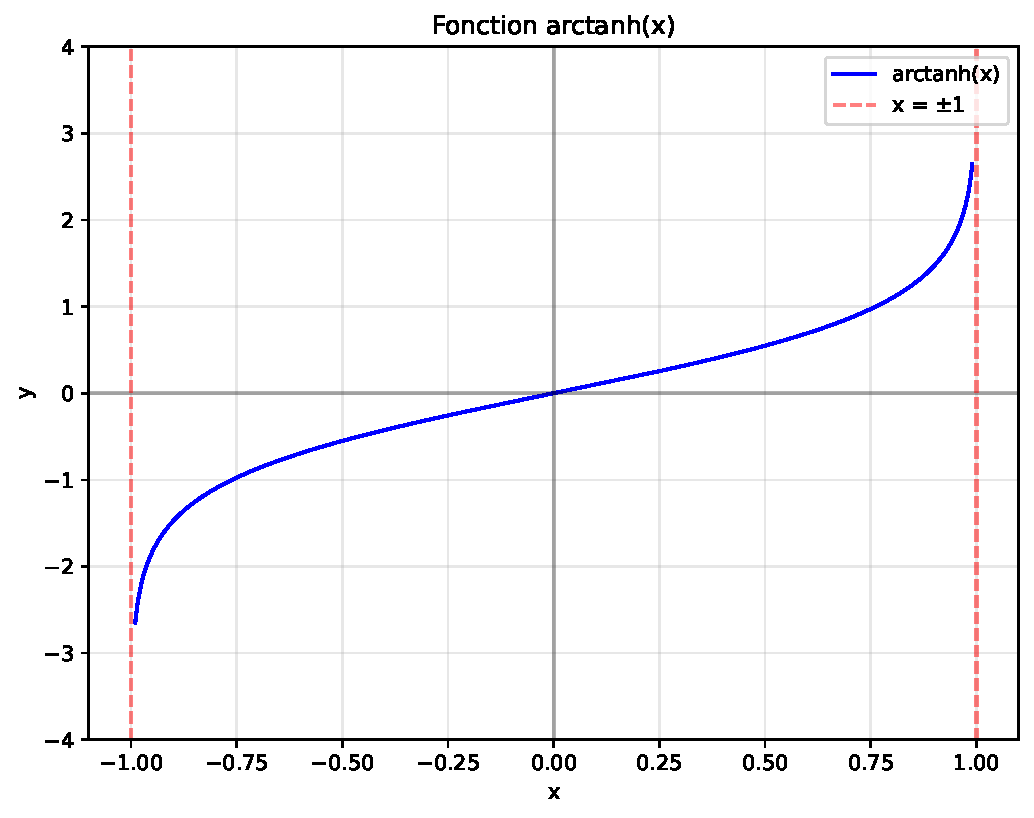
\includegraphics{exercices/FonctionsHyp/FonctionsHyp_files/figure-pdf/cell-3-output-1.pdf}

  }

  \end{figure}

  \end{solution}
\end{enumerate}

\hypertarget{question-2-3}{%
\section{Question 2}\label{question-2-3}}

Exprimez \(\cosh(x+y)\) en fonction de \(\cosh x\), \(\cosh y\),
\(\sinh x\) et \(\sinh y\).

\begin{solution}

Exprimons \(\cosh(x+y)\) en fonction de \(\cosh x\), \(\cosh y\),
\(\sinh x\) et \(\sinh y\). Rappelons que \(\cosh(x+y)\) peut s'écrire
en utilisant la forme exponentielle
\[\cosh(x+y) = \frac{e^{x+y} + e^{-(x+y)}}{2}.\] Développons \(e^{x+y}\)
et \(e^{-(x+y)}\) : \[\cosh(x+y) = \frac{e^x e^y + e^{-x} e^{-y}}{2}.\]

Rappelons les formules :
\[\cosh x = \frac{e^x + e^{-x}}{2} \quad \text{et} \quad \sinh x = \frac{e^x - e^{-x}}{2}.\]
Donc :
\[e^x = \cosh x + \sinh x \quad \text{et} \quad e^{-x} = \cosh x - \sinh x\]
Substituons ces expressions dans notre équation :
\[\cosh(x+y) = \frac{(\cosh x + \sinh x)(\cosh y + \sinh y) + (\cosh x - \sinh x)(\cosh y - \sinh y)}{2}.\]
Développons les produits : \begin{align}
\cosh(x+y) &= \frac{1}{2}\left(\cosh x \cosh y + \sinh x \cosh y + \cosh x \sinh y + \sinh x \sinh y + \cosh x \cosh y\right.\\
&~\left.- \sinh x \cosh y - \cosh x \sinh y + \sinh x \sinh y\right).
\end{align} Regroupons les termes semblables :
\[\cosh(x+y) = \frac{2\cosh x \cosh y + 2\sinh x \sinh y}{2}\]
Simplifions : \[\cosh(x+y) = \cosh x \cosh y + \sinh x \sinh y\] Nous
avons donc la formule cherchée :
\(\cosh(x+y) = \cosh x \cosh y + \sinh x \sinh y\).

\end{solution}

\hypertarget{question-3-3}{%
\section{Question 3}\label{question-3-3}}

\begin{enumerate}
\def\labelenumi{\arabic{enumi}.}
\item
  Résolvez l'équation \(\sinh(2x) = 3\).
\item
  En déduire les solutions de l'équation \(\cosh(2x) = \sqrt{10}\).
\item
  Ces deux équations sont-elles liées ? Justifier votre réponse.
\end{enumerate}

\begin{solution}

\begin{enumerate}
\def\labelenumi{\arabic{enumi}.}
\item
  Par définition, \[\sinh(2x) = \dfrac{e^{2x} - e^{-2x}}{2} = 3.\] On en
  déduit que \(e^{2x} - e^{-2x} = 6\). Posons \(y = e^{2x}\). Ainsi,
  \(y - \frac{1}{y} = 6\), d'où \(y^2 - 6y - 1 = 0\). On en déduit que
  \[y = 3\pm \sqrt{10}.\] Comme \(e^{2x} > 0\), on déduit que
  \(e^{2x} = 3 + \sqrt{10}\). En prenant le logarithme, on arrive à
  isoler \(x\) pour obtenir
  \[x = \frac{1}{2}\ln\left(3 + \sqrt{10}\right).\]
\item
  Utilisons l'identité \(\cosh^2(x) - \sinh^2(x) = 1\), valable pour
  toute valeur de \(x\). Si \(\sinh(2x) = 3\), alors
  \(\cosh^2(2x) = 10\). Ainsi, \(\cosh(2x) = \pm\sqrt{10}\). Comme
  \(\cosh(x) \geq 1\) pour tout \(x\), \(\cosh(2x) = \sqrt{10}\). On
  trouve la même solution, à savoir
  \[x = \frac{1}{2}\ln\left(3 + \sqrt{10}\right).\]
\item
  Ces équations sont liées par l'identité
  \(\cosh^2(x) - \sinh^2(x) = 1\). Quand on connaît \(\sinh(2x)\), on
  peut déduire \(\cosh(2x)\). Les solutions sont les mêmes car
  \(\sinh(x)\) et \(\cosh(x)\) sont liés.
\end{enumerate}

\end{solution}

\hypertarget{question-4-3}{%
\section{Question 4}\label{question-4-3}}

Tracer sur un même graphique les fonctions \(f(x) = \sinh(x)\) et
\(g(x) = \cosh(x)\).

\begin{solution}

\begin{Shaded}
\begin{Highlighting}[]
\ImportTok{import}\NormalTok{ numpy }\ImportTok{as}\NormalTok{ np}
\ImportTok{import}\NormalTok{ matplotlib.pyplot }\ImportTok{as}\NormalTok{ plt}

\CommentTok{\# Création des données}
\NormalTok{x }\OperatorTok{=}\NormalTok{ np.linspace(}\OperatorTok{{-}}\DecValTok{4}\NormalTok{, }\DecValTok{4}\NormalTok{, }\DecValTok{1000}\NormalTok{)}
\NormalTok{sinh }\OperatorTok{=}\NormalTok{ np.sinh(x)}
\NormalTok{cosh }\OperatorTok{=}\NormalTok{ np.cosh(x)}

\CommentTok{\# Création du graphique}
\NormalTok{plt.figure(figsize}\OperatorTok{=}\NormalTok{(}\DecValTok{8}\NormalTok{, }\DecValTok{8}\NormalTok{))}
\NormalTok{plt.plot(x, sinh, }\StringTok{\textquotesingle{}b{-}\textquotesingle{}}\NormalTok{, label}\OperatorTok{=}\StringTok{\textquotesingle{}sinh(x)\textquotesingle{}}\NormalTok{)}
\NormalTok{plt.plot(x, cosh, }\StringTok{\textquotesingle{}r{-}\textquotesingle{}}\NormalTok{, label}\OperatorTok{=}\StringTok{\textquotesingle{}cosh(x)\textquotesingle{}}\NormalTok{)}

\CommentTok{\# Configuration du graphique}
\NormalTok{plt.grid(}\VariableTok{True}\NormalTok{, alpha}\OperatorTok{=}\FloatTok{0.3}\NormalTok{)}
\NormalTok{plt.title(}\StringTok{\textquotesingle{}Fonctions hyperboliques\textquotesingle{}}\NormalTok{)}
\NormalTok{plt.xlabel(}\StringTok{\textquotesingle{}x\textquotesingle{}}\NormalTok{)}
\NormalTok{plt.ylabel(}\StringTok{\textquotesingle{}y\textquotesingle{}}\NormalTok{)}
\NormalTok{plt.legend()}
\NormalTok{plt.axhline(y}\OperatorTok{=}\DecValTok{0}\NormalTok{, color}\OperatorTok{=}\StringTok{\textquotesingle{}k\textquotesingle{}}\NormalTok{, linestyle}\OperatorTok{=}\StringTok{\textquotesingle{}{-}\textquotesingle{}}\NormalTok{, alpha}\OperatorTok{=}\FloatTok{0.3}\NormalTok{)}
\NormalTok{plt.axvline(x}\OperatorTok{=}\DecValTok{0}\NormalTok{, color}\OperatorTok{=}\StringTok{\textquotesingle{}k\textquotesingle{}}\NormalTok{, linestyle}\OperatorTok{=}\StringTok{\textquotesingle{}{-}\textquotesingle{}}\NormalTok{, alpha}\OperatorTok{=}\FloatTok{0.3}\NormalTok{)}

\NormalTok{plt.show()}
\end{Highlighting}
\end{Shaded}

\begin{figure}[H]

{\centering 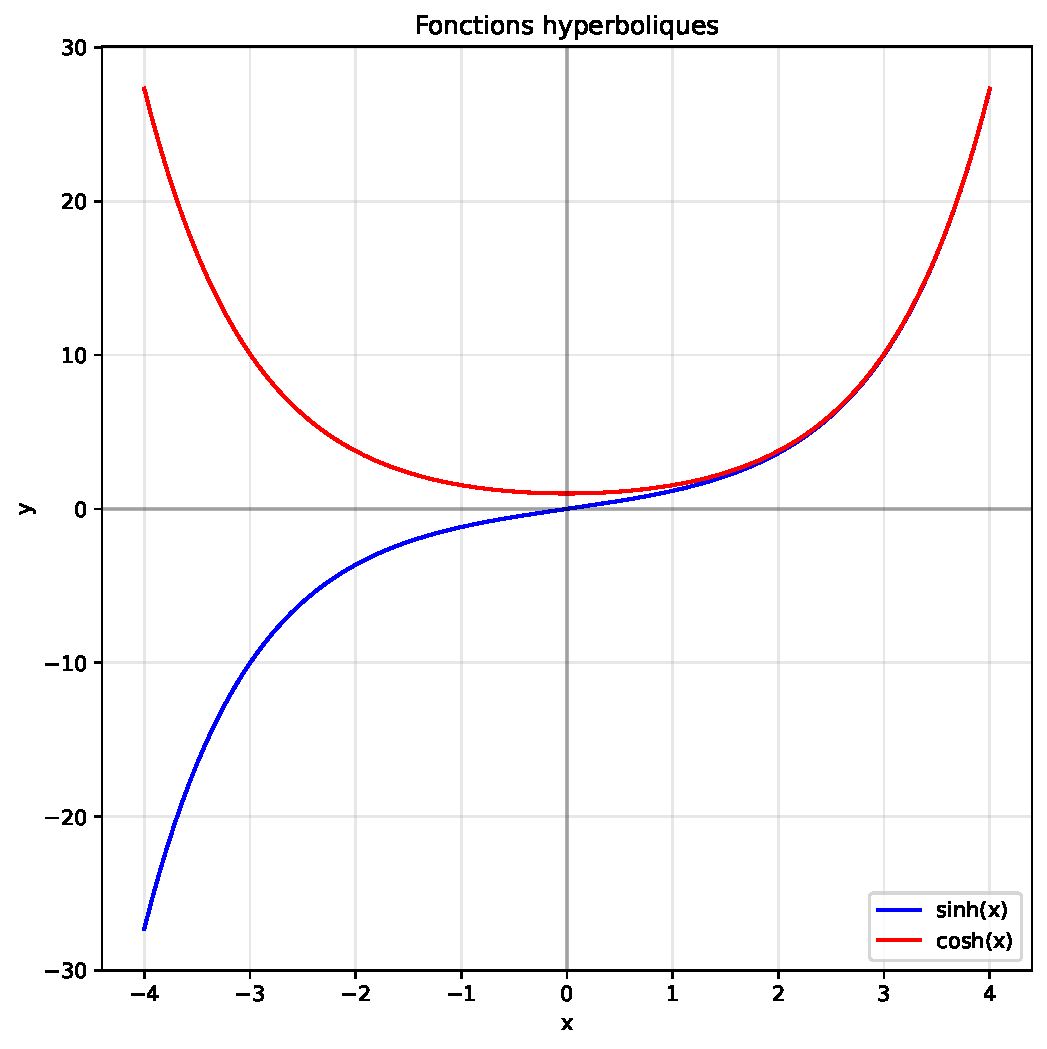
\includegraphics{exercices/FonctionsHyp/FonctionsHyp_files/figure-pdf/cell-4-output-1.pdf}

}

\end{figure}

\textbf{Analyse du graphique} 1. La fonction \(\sinh(x)\) : * Est
impaire * Passe par l'origine * N'atteint pas de maximum ni de minimum

\begin{enumerate}
\def\labelenumi{\arabic{enumi}.}
\setcounter{enumi}{1}
\tightlist
\item
  La fonction \(\cosh(x)\) :

  \begin{itemize}
  \tightlist
  \item
    Est paire
  \item
    A un minimum de \(1\) en \(x = 0\)
  \item
    Ne possède pas de maximum
  \end{itemize}
\end{enumerate}

\end{solution}

\hypertarget{question-5-3}{%
\section{Question 5}\label{question-5-3}}

Démontrer les identités suivantes :

\begin{enumerate}
\def\labelenumi{\arabic{enumi}.}
\item
  \(\sinh(x+y) = \sinh(x)\cosh(y) + \cosh(x)\sinh(y)\)
\item
  \(\tanh(x) + \tanh(y) = \frac{\sinh(x+y)}{\cosh(x)\cosh(y)}\)
\end{enumerate}

\begin{solution}

\begin{enumerate}
\def\labelenumi{\arabic{enumi}.}
\item
  Démarche semblable à celle exigée à la question 2.
\item
  Nous avons que \begin{align}
  \tanh(x) + \tanh(y) &= \frac{\sinh(x)}{\cosh(x)} + \frac{\sinh(y)}{\cosh(y)}\\
  &= \frac{\sinh(x)\cosh(y) + \cosh(x)\sinh(y)}{\cosh(x)\cosh(y)}\\
  &= \frac{\sinh(x+y)}{\cosh(x)\cosh(y)}\qquad\text{(d'après (a)).}
  \end{align}
\end{enumerate}

\end{solution}

\hypertarget{question-6-3}{%
\section{Question 6}\label{question-6-3}}

Un câble pesant est suspendu entre deux points situés à une hauteur
commune de 50 mètres et distants de 10 mètres. Le point le plus bas du
câble est à 10 mètres sous les points de suspension. Trouvez l'équation
de la chaînette passant par ces points. Remarques : vous pouvez supposer
que la droite \(x=0\) est un axe de symétrie de la chaînette. Aussi,
vous aurez besoin d'utiliser un logiciel pour calculer un des
paramètres.

\begin{solution}

La solution sera présentée en classe.

\end{solution}

L'équation d'une chaînette est de la forme
\(y = a \cosh(\frac{x}{a}) + k\). Les points de suspension sont en
\((-5,0)\) et \((5,0)\) et le point le plus bas est en \((0,-2)\).
Ainsi, nous obtenons les équations \begin{align}
-2 &= a \cosh(0) + k,\\
0 &= a \cosh(5/a) + k.
\end{align} \begin{align}
-2 &= a + k,\\
0 &= a \cosh(5/a) + -2-a.
\end{align}

L'équation \(0 = a \cosh(5/a) + -2-a\) se résout numériquement (par
exemple avec WolframAlpha). On trouve que \(a \approx 3.95\). On en
déduit ensuite que \(k\approx -5.95\). Ainsi, l'équation de la chaînette
est \[y = 3.95 \cosh\left(\frac{x}{3.95}\right) - 5.95.\]

\begin{Shaded}
\begin{Highlighting}[]
\ImportTok{import}\NormalTok{ numpy }\ImportTok{as}\NormalTok{ np}
\ImportTok{import}\NormalTok{ matplotlib.pyplot }\ImportTok{as}\NormalTok{ plt}

\CommentTok{\# Paramètres}
\NormalTok{a }\OperatorTok{=} \FloatTok{3.95}
\NormalTok{k }\OperatorTok{=} \OperatorTok{{-}}\FloatTok{5.95}

\CommentTok{\# Points}
\NormalTok{x }\OperatorTok{=}\NormalTok{ np.linspace(}\OperatorTok{{-}}\DecValTok{5}\NormalTok{, }\DecValTok{5}\NormalTok{, }\DecValTok{1000}\NormalTok{)}
\NormalTok{y }\OperatorTok{=}\NormalTok{ a }\OperatorTok{*}\NormalTok{ np.cosh(x}\OperatorTok{/}\NormalTok{a) }\OperatorTok{+}\NormalTok{ k}

\CommentTok{\# Graphique}
\NormalTok{plt.figure(figsize}\OperatorTok{=}\NormalTok{(}\DecValTok{8}\NormalTok{, }\DecValTok{6}\NormalTok{))}
\NormalTok{plt.plot(x, y, }\StringTok{\textquotesingle{}b{-}\textquotesingle{}}\NormalTok{, label}\OperatorTok{=}\StringTok{\textquotesingle{}Chaînette\textquotesingle{}}\NormalTok{)}
\NormalTok{plt.grid(}\VariableTok{True}\NormalTok{)}
\NormalTok{plt.axis(}\StringTok{\textquotesingle{}equal\textquotesingle{}}\NormalTok{)}
\NormalTok{plt.title(}\StringTok{\textquotesingle{}Câble suspendu (chaînette)\textquotesingle{}}\NormalTok{)}
\NormalTok{plt.xlabel(}\StringTok{\textquotesingle{}x (m)\textquotesingle{}}\NormalTok{)}
\NormalTok{plt.ylabel(}\StringTok{\textquotesingle{}y (m)\textquotesingle{}}\NormalTok{)}
\NormalTok{plt.legend()}
\NormalTok{plt.show()}
\end{Highlighting}
\end{Shaded}

\begin{figure}[H]

{\centering 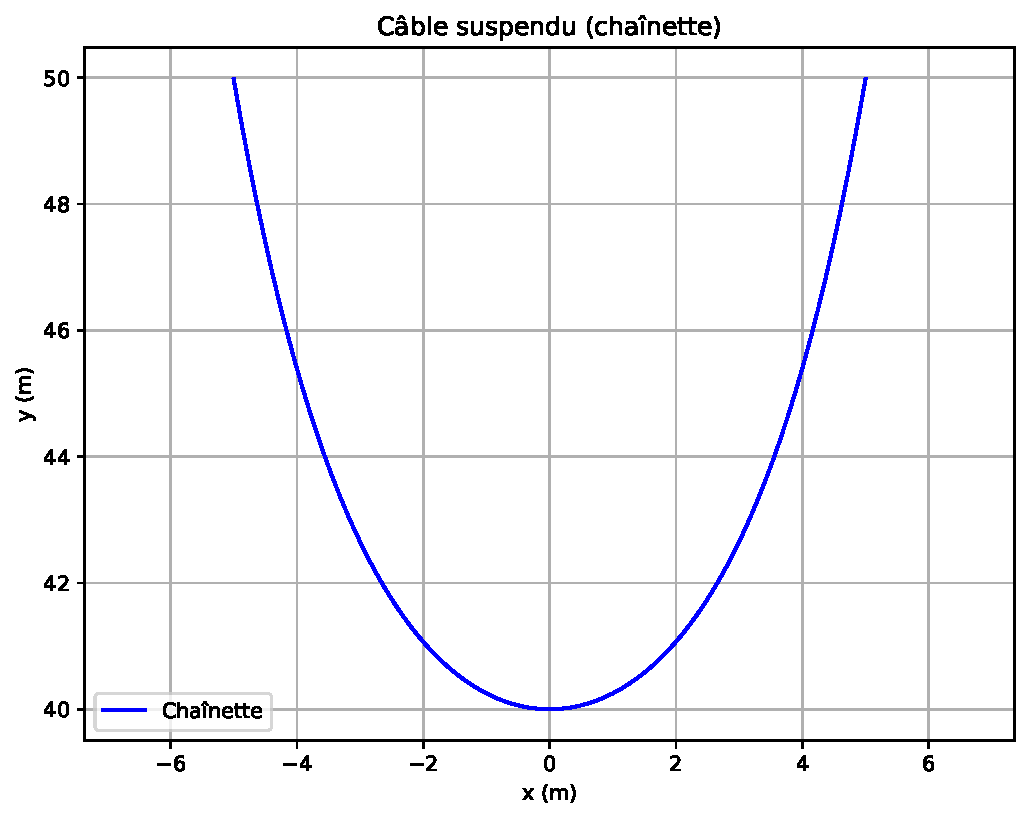
\includegraphics{exercices/FonctionsHyp/FonctionsHyp_files/figure-pdf/cell-5-output-1.pdf}

}

\end{figure}

\begin{enumerate}
\def\labelenumi{\alph{enumi})}
\setcounter{enumi}{1}
\tightlist
\item
  La longueur du câble est donnée par :
  \(L = 2a \sinh(5/a) \approx 10.49\) mètres
\end{enumerate}

\hypertarget{les-uxe9quations-diffuxe9rentielles}{%
\chapter{Les équations
différentielles}\label{les-uxe9quations-diffuxe9rentielles}}

\hypertarget{question-1-4}{%
\section{Question 1}\label{question-1-4}}

Résoudre l'équation différentielle : \(\frac{dy}{dx} = 2xy\)

\begin{solution}

D'abord, on réorganise l'équation comme \(\frac{1}{y}dy = 2x dx\). Nous
avons divisé par \(y\), que nous supposons différente de la fonction
identiquement nulle pour la suite. Remarquons que la fonction
identiquement nulle est une solution de l'équation différentielle.

Intégrons les deux membres de l'équation :
\(\int \frac{1}{y}dy = \int 2x dx\). Nous obtenons
que\(\ln|y| = x^2 + C\). En prenant l'exponentielle, nous obtenons que
\(|y|=e^{C}e^{x^2}\). Ainsi, \(|y|=C_1e^{x^2}\), où \(C_1\) est une
constante strictement positive. De là nous avons que \(y=C_2e^{x^2}\),
où \(C_2\) est une constante réelle non nulle. Finalement, on se
rappelle que \(y=0\) est solution de l'équation différentielle de
départ, ce qui nous permet d'écrire que l'ensemble des solutions de
l'équation différentielle est formé de toutes les fonctions de la forme
\(y=Ke^{x^2}, K\in\mathbb{R}\).

\end{solution}

\hypertarget{question-2-4}{%
\section{Question 2}\label{question-2-4}}

Résoudre l'équation différentielle \[\frac{dy}{dx} = \frac{x}{y}.\]

\begin{solution}

On sépare les variables pour obtenir l'équation \(y dy = x dx\). On
intègre ensuite les deux membres de l'équation :
\(\int y dy = \int x dx\). Nous obtenons que
\(\frac{y^2}{2} = \frac{x^2}{2} + C\). Ainsi, la solution générale est
\[y = \pm\sqrt{x^2 + K},\] où \(K\) est une constante arbitraire.

\end{solution}

\hypertarget{question-3-4}{%
\section{Question 3}\label{question-3-4}}

Résoudre l'équation différentielle \[\frac{dy}{dx} = \frac{y}{x}.\]

\begin{solution}

On sépare les variables pour obtenir l'équation
\(\frac{dy}{y} = \frac{dx}{x}\). On a divisé par \(y\), on supposera
donc pour la suite que \(y\) n'est pas identiquement nulle. On remarque
aussi que la fonction identiquement nulle est une solution de l'équation
différentielle.

On intègre ensuite les deux membres de l'équation :
\(\int \frac{dy}{y} = \int \frac{dx}{x}\). Nous obtenons que
\(\ln|y| = \ln|x| + C\). Comme la fonction \(\ln\) est une bijection des
réels strictement positifs vers \(\mathbb{R}\), il existe un unique
\(k\in\mathbb{R}_{>0}\) tel que \(C=\ln k\). Ainsi,
\[\ln|y| = \ln|x| + C=\ln|x| + \ln k=\ln k|x|.\] L'injectivité de la
fonction \(\ln\) implique que \(y=\pm k|x|\). Si on trace ces courbes,
on constate qu'il s'agit des droites de pente non nulle passant par
l'origine. Comme la droite \(y(x)=0\) est une solution (on l'a remarqué
plus tôt), l'ensemble des solutions consiste à être l'ensemble des
droites passant par l'origine, c'est-à-dire aux courbes d'équation
\(y(x)=Dx, D\in\mathbb{R}\).

\end{solution}

\hypertarget{question-4-4}{%
\section{Question 4}\label{question-4-4}}

Résoudre l'équation différentielle : \(\frac{dy}{dx} = y^2\)

\begin{solution}

On constate que \(y(x)=0\) est une solution. Maintenant, pour trouver
les solutions non nulles, divisons par \(y^2\) pour séparer les
variables. On obtient ainsi que \[\frac{dy}{y^2} = dx.\] En intégrant
chacun des membres de l'équation, nous obtenons que
\[-\frac{1}{y} = x + C,\] où \(C\) est une constante réelle arbitraire.
On isole par la suite \(y\), pour obtenir une solution de la forme
\[y = -\frac{1}{x + K},\] où \(K\) est une constante réelle arbitraire.

\end{solution}

\hypertarget{question-5-4}{%
\section{Question 5}\label{question-5-4}}

Résoudre l'équation différentielle : \(\frac{dy}{dx} = e^{x-y}\)

\begin{solution}

Pour résoudre cette équation, commençons par réorganiser les termes afin
de séparer les variables. En multipliant chaque membre par \(e^y\), nous
obtenons \[e^y dy = e^x dx.\] En intégrant chacun des membres de
l'équation, nous obtenons que \[e^y = e^x + C,\] où \(C\) est une
constante réelle arbitraire. On isole par la suite \(y\) en appliquant
le logarithme naturel de chaque côté, pour obtenir une solution de la
forme \[y(x) = \ln(e^x + C).\]

\end{solution}

\hypertarget{question-6-4}{%
\section{Question 6}\label{question-6-4}}

Lorsqu'une personne avale une substance toxique, son foie tente de
l'éliminer. Généralement, le taux d'élimination de la quantité de
substance encore présente dans l'organisme au temps \(t\) --- que nous
noterons \(Q(t)\) --- est proportionnel à la quantité de substance
encore présente dans l'organisme au temps \(t\). Au temps \(t=0\),
Jocelyn a avalé une quantité \(Q_0\) d'un liquide toxique. Après 3
heures, on a estimé que son foie avait éliminé 50\% du liquide. D'après
ce modèle, combien d'heures se seront écoulées entre le moment où
Jocelyn a avalé le produit et celui où il en aura éliminé 90\%?

\hypertarget{question-7-2}{%
\section{Question 7}\label{question-7-2}}

Un vêtement pesant 50 grammes est plongée dans un bassin d'eau. En le
sortant du bassin, au temps \(t=0\), sa masse est de 200 grammes. On
l'étend immédiatement sur une corde à linge pour qu'il sèche. On observe
qu'après 180 minutes, sa masse est de 100 grammes. Combien de minutes se
seront écoulées entre le moment où le vêtement est sorti du bassin et
celui où il aura évacué 99\% de l'eau qu'il contenait initialement?
Arrondissez à la minute. Pour répondre à cette question, on fera
l'hypothèse que le taux d'évaporation d'eau dans le vêtement est
proportionnel à la quantité d'eau présente dans celui-ci.

\hypertarget{question-8-2}{%
\section{Question 8}\label{question-8-2}}

Un réservoir contient initialement 100 kg de lait écrémé (le pourcentage
de matière grasse du lait écrémé est de 0 \%). Au temps \(t=0\), on
commence à y verser, à un taux constant de 10 kg/minute, du lait dont le
pourcentage de matière grasse est de 4 \%. Au même moment, un drain
évacue le lait du réservoir vers le camion réfrigérée, à un taux
constant de 10 kg/minute. Pour répondre à cette question, on fera
l'hypothèse que le mélangeur du réservoir permet de garder son contenu
homogène.

\begin{enumerate}
\tightlist
\item
  Soit \(M\) la masse (en kg) de matière grasse dans le réservoir en
  fonction du temps \(t\) (en minutes). Trouvez la fonction \(M(t)\).
\item
  Évaluez \(\lim_{t\rightarrow\infty}M(t)\).
\end{enumerate}

\begin{solution}

\begin{enumerate}
\item
  Pendant un petit intervalle de temps \(\Delta t\) minutes, il entre
  10\(\Delta t\) kilogrammes de lait, qui contient une proportion 4/100
  de matières grasses. Donc la masse de matières grasses entrant est
  \[M_{\text{entrant}} = \frac{4}{100} \times 10\Delta t = 0{,}4 \Delta t\]

  Pendant le même intervalle, il sort une masse \(10\Delta t\) de lait.
  La proportion de matières grasses dans ce lait est \(M(t)/100\).
  Ainsi, on a
  \[M_{\text{entrant}} = \frac{M(t)}{100} \times 10\Delta t = \frac{M(t)}{10} \Delta t.\]

  Le changement dans \(M(t)\) est donc
  \[\Delta M = M_{\text{entrant}} - M_{\text{sortant}} = 0{,}4 \Delta t - \frac{M(t)}{10} \Delta t.\]
  Ainsi \[\frac{\Delta M}{\Delta t} = 0{,}4 - \frac{M(t)}{10}.\] Quand
  \(\Delta t\) tend vers 0, le membre de gauche tend vers \(M'(t)\), et
  on obtient \[M'(t) = 0{,}4 - \frac{M(t)}{10}.\] Cette équation est
  séparable. On a \[\frac{dM}{0{,}4 - \frac{M}{10}} = dt,\] qui est
  équivalente à \[\int \frac{10dM}{4 - M} = \int dt.\] On intègre et on
  obtient que \[-10 \ln|4 - M| = t + C,\] équation qui est équivalente à
  \[|4 - M| = ke^{-t/10}.\] Puisque \(M(0) = 0\), on en déduit que
  \(k = 4\) et finalement \[M(t) = 4 - 4e^{-t/10}.\]
\item
  Puisque \(e^{-t/10} \to 0\) quand \(t \to \infty\), on a
  \(\lim_{t \to \infty} M(t) = 4\). Intuitivement, ce résultat est
  évident car à la longue, on s'attend à ce que l'état initial devienne
  négligeable et que la proportion de gras dans le lait du réservoir
  soit la même que celle du lait qu'on y ajoute.
\end{enumerate}

\end{solution}

\part{Problèmes résolus}

\hypertarget{le-ballon-muxe9tuxe9orologique}{%
\chapter{Le ballon
météorologique}\label{le-ballon-muxe9tuxe9orologique}}

Un ballon est lancé verticalement vers le haut avec une vitesse initiale
de 10 m/s. En tenant compte de la résistance de l'air, sa hauteur (en
mètres) après \(t\) secondes est donnée par la fonction :

\[h(t) = 50\ln(\cosh(0.2t)) + 10t - 4.9t^2\]

À quel moment le ballon atteint-il son altitude maximale ?

\hypertarget{visualisation-du-probluxe8me}{%
\subsection{1. Visualisation du
problème}\label{visualisation-du-probluxe8me}}

Commençons par visualiser la hauteur du ballon en fonction du temps :

\begin{Shaded}
\begin{Highlighting}[]
\FunctionTok{library}\NormalTok{(ggplot2)}
\FunctionTok{library}\NormalTok{(dplyr)}
\end{Highlighting}
\end{Shaded}

\begin{verbatim}

Attaching package: 'dplyr'
\end{verbatim}

\begin{verbatim}
The following objects are masked from 'package:stats':

    filter, lag
\end{verbatim}

\begin{verbatim}
The following objects are masked from 'package:base':

    intersect, setdiff, setequal, union
\end{verbatim}

\begin{Shaded}
\begin{Highlighting}[]
\CommentTok{\# Fonction hauteur}
\NormalTok{h }\OtherTok{\textless{}{-}} \ControlFlowTok{function}\NormalTok{(t) \{}
  \DecValTok{50} \SpecialCharTok{*} \FunctionTok{log}\NormalTok{(}\FunctionTok{cosh}\NormalTok{(}\FloatTok{0.2} \SpecialCharTok{*}\NormalTok{ t)) }\SpecialCharTok{+} \DecValTok{10} \SpecialCharTok{*}\NormalTok{ t }\SpecialCharTok{{-}} \FloatTok{4.9} \SpecialCharTok{*}\NormalTok{ t}\SpecialCharTok{\^{}}\DecValTok{2}
\NormalTok{\}}

\CommentTok{\# Création des données}
\NormalTok{t\_vals }\OtherTok{\textless{}{-}} \FunctionTok{seq}\NormalTok{(}\DecValTok{0}\NormalTok{, }\DecValTok{3}\NormalTok{, }\AttributeTok{by =} \FloatTok{0.01}\NormalTok{)}
\NormalTok{height\_data }\OtherTok{\textless{}{-}} \FunctionTok{data.frame}\NormalTok{(}
  \AttributeTok{t =}\NormalTok{ t\_vals,}
  \AttributeTok{height =} \FunctionTok{sapply}\NormalTok{(t\_vals, h)}
\NormalTok{)}

\CommentTok{\# Graphique}
\FunctionTok{ggplot}\NormalTok{(height\_data, }\FunctionTok{aes}\NormalTok{(}\AttributeTok{x =}\NormalTok{ t, }\AttributeTok{y =}\NormalTok{ height)) }\SpecialCharTok{+}
  \FunctionTok{geom\_line}\NormalTok{(}\AttributeTok{color =} \StringTok{"blue"}\NormalTok{, }\AttributeTok{size =} \DecValTok{1}\NormalTok{) }\SpecialCharTok{+}
  \FunctionTok{labs}\NormalTok{(}\AttributeTok{x =} \StringTok{"Temps (s)"}\NormalTok{, }\AttributeTok{y =} \StringTok{"Hauteur (m)"}\NormalTok{) }\SpecialCharTok{+}
  \FunctionTok{theme\_minimal}\NormalTok{() }\SpecialCharTok{+}
  \FunctionTok{ggtitle}\NormalTok{(}\StringTok{"Trajectoire du ballon"}\NormalTok{)}
\end{Highlighting}
\end{Shaded}

\begin{verbatim}
Warning: Using `size` aesthetic for lines was deprecated in ggplot2 3.4.0.
i Please use `linewidth` instead.
\end{verbatim}

\begin{figure}[H]

{\centering 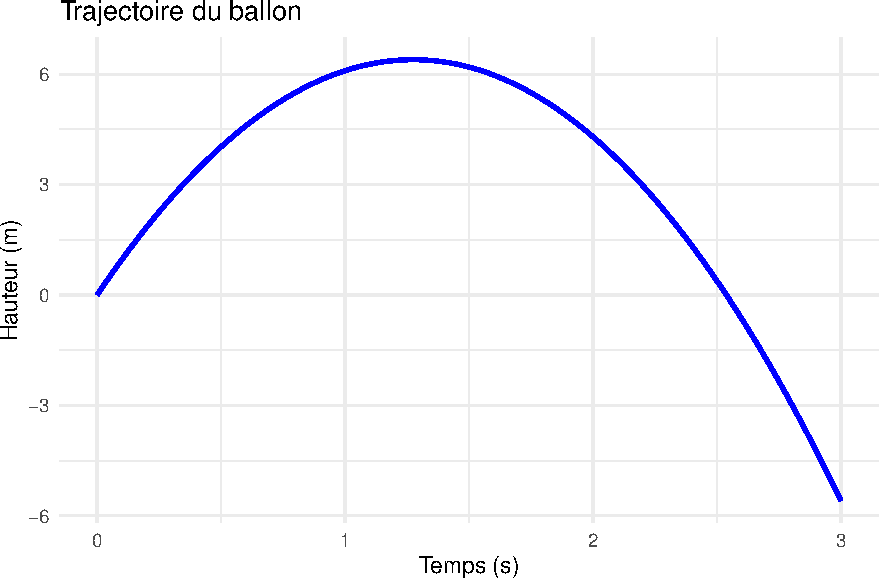
\includegraphics{theorie/pi/ballonmeteo_files/figure-pdf/fig-hauteur-1.pdf}

}

\caption{\label{fig-hauteur}Hauteur du ballon en fonction du temps}

\end{figure}

\hypertarget{la-vitesse-du-ballon}{%
\subsection{2. La vitesse du ballon}\label{la-vitesse-du-ballon}}

La vitesse est la dérivée de la hauteur. Pour trouver le point
culminant, nous devons trouver quand la vitesse est nulle.

\[v(t) = h'(t) = 10\tanh(0.2t) + 10 - 9.8t\]

Visualisons la vitesse :

\begin{Shaded}
\begin{Highlighting}[]
\CommentTok{\# Fonction vitesse}
\NormalTok{v }\OtherTok{\textless{}{-}} \ControlFlowTok{function}\NormalTok{(t) \{}
  \DecValTok{10} \SpecialCharTok{*} \FunctionTok{tanh}\NormalTok{(}\FloatTok{0.2} \SpecialCharTok{*}\NormalTok{ t) }\SpecialCharTok{+} \DecValTok{10} \SpecialCharTok{{-}} \FloatTok{9.8} \SpecialCharTok{*}\NormalTok{ t}
\NormalTok{\}}

\CommentTok{\# Création des données}
\NormalTok{velocity\_data }\OtherTok{\textless{}{-}} \FunctionTok{data.frame}\NormalTok{(}
  \AttributeTok{t =}\NormalTok{ t\_vals,}
  \AttributeTok{velocity =} \FunctionTok{sapply}\NormalTok{(t\_vals, v)}
\NormalTok{)}

\CommentTok{\# Graphique}
\FunctionTok{ggplot}\NormalTok{(velocity\_data, }\FunctionTok{aes}\NormalTok{(}\AttributeTok{x =}\NormalTok{ t, }\AttributeTok{y =}\NormalTok{ velocity)) }\SpecialCharTok{+}
  \FunctionTok{geom\_line}\NormalTok{(}\AttributeTok{color =} \StringTok{"red"}\NormalTok{, }\AttributeTok{size =} \DecValTok{1}\NormalTok{) }\SpecialCharTok{+}
  \FunctionTok{geom\_hline}\NormalTok{(}\AttributeTok{yintercept =} \DecValTok{0}\NormalTok{, }\AttributeTok{linetype =} \StringTok{"dashed"}\NormalTok{) }\SpecialCharTok{+}
  \FunctionTok{labs}\NormalTok{(}\AttributeTok{x =} \StringTok{"Temps (s)"}\NormalTok{, }\AttributeTok{y =} \StringTok{"Vitesse (m/s)"}\NormalTok{) }\SpecialCharTok{+}
  \FunctionTok{theme\_minimal}\NormalTok{() }\SpecialCharTok{+}
  \FunctionTok{ggtitle}\NormalTok{(}\StringTok{"Vitesse du ballon"}\NormalTok{)}
\end{Highlighting}
\end{Shaded}

\begin{figure}[H]

{\centering 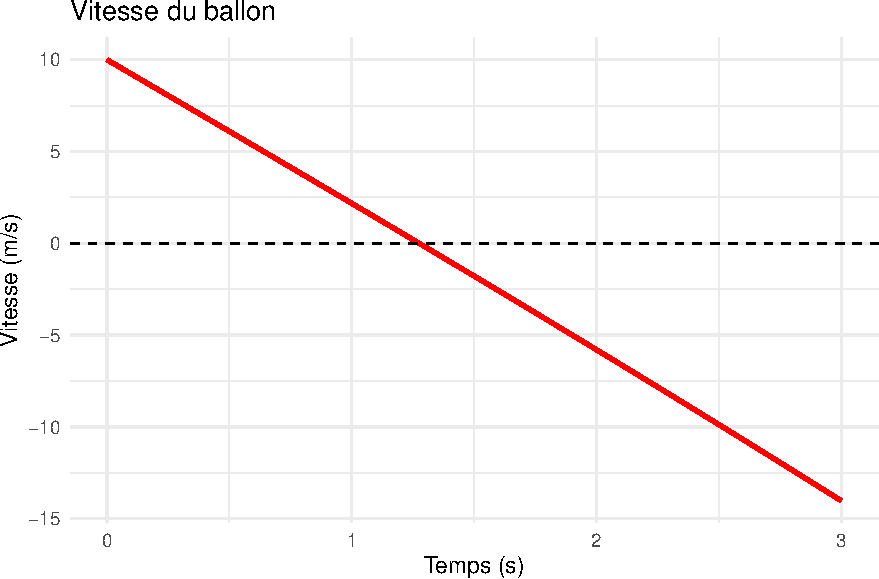
\includegraphics{theorie/pi/ballonmeteo_files/figure-pdf/fig-vitesse-1.pdf}

}

\caption{\label{fig-vitesse}Vitesse du ballon en fonction du temps}

\end{figure}

\hypertarget{muxe9thode-de-newton-raphson}{%
\subsection{3. Méthode de
Newton-Raphson}\label{muxe9thode-de-newton-raphson}}

Pour trouver quand la vitesse est nulle, nous devons résoudre :
\[f(t) = 10\tanh(0.2t) + 10 - 9.8t = 0\]

La dérivée de cette fonction est :
\[f'(t) = 2\,\text{sech}^2(0.2t) - 9.8\]

Implémentons la méthode de Newton-Raphson :

\begin{Shaded}
\begin{Highlighting}[]
\CommentTok{\# Fonction f(t) et sa dérivée}
\NormalTok{f }\OtherTok{\textless{}{-}} \ControlFlowTok{function}\NormalTok{(t) \{}
  \DecValTok{10} \SpecialCharTok{*} \FunctionTok{tanh}\NormalTok{(}\FloatTok{0.2} \SpecialCharTok{*}\NormalTok{ t) }\SpecialCharTok{+} \DecValTok{10} \SpecialCharTok{{-}} \FloatTok{9.8} \SpecialCharTok{*}\NormalTok{ t}
\NormalTok{\}}

\NormalTok{f\_prime }\OtherTok{\textless{}{-}} \ControlFlowTok{function}\NormalTok{(t) \{}
  \DecValTok{2} \SpecialCharTok{*}\NormalTok{ (}\DecValTok{1} \SpecialCharTok{/} \FunctionTok{cosh}\NormalTok{(}\FloatTok{0.2} \SpecialCharTok{*}\NormalTok{ t))}\SpecialCharTok{\^{}}\DecValTok{2} \SpecialCharTok{{-}} \FloatTok{9.8}
\NormalTok{\}}

\CommentTok{\# Fonction Newton{-}Raphson}
\NormalTok{newton\_raphson }\OtherTok{\textless{}{-}} \ControlFlowTok{function}\NormalTok{(x0, }\AttributeTok{tolerance =} \FloatTok{1e{-}6}\NormalTok{, }\AttributeTok{max\_iter =} \DecValTok{100}\NormalTok{) \{}
\NormalTok{  x }\OtherTok{\textless{}{-}}\NormalTok{ x0}
\NormalTok{  iterations }\OtherTok{\textless{}{-}} \FunctionTok{data.frame}\NormalTok{(}
    \AttributeTok{iteration =} \DecValTok{0}\NormalTok{,}
    \AttributeTok{x =}\NormalTok{ x0,}
    \AttributeTok{f\_x =} \FunctionTok{f}\NormalTok{(x0)}
\NormalTok{  )}
  
  \ControlFlowTok{for}\NormalTok{ (i }\ControlFlowTok{in} \DecValTok{1}\SpecialCharTok{:}\NormalTok{max\_iter) \{}
\NormalTok{    x\_new }\OtherTok{\textless{}{-}}\NormalTok{ x }\SpecialCharTok{{-}} \FunctionTok{f}\NormalTok{(x) }\SpecialCharTok{/} \FunctionTok{f\_prime}\NormalTok{(x)}
    
\NormalTok{    iterations }\OtherTok{\textless{}{-}} \FunctionTok{rbind}\NormalTok{(iterations, }
                       \FunctionTok{data.frame}\NormalTok{(}\AttributeTok{iteration =}\NormalTok{ i,}
                                \AttributeTok{x =}\NormalTok{ x\_new,}
                                \AttributeTok{f\_x =} \FunctionTok{f}\NormalTok{(x\_new)))}
    
    \ControlFlowTok{if}\NormalTok{ (}\FunctionTok{abs}\NormalTok{(x\_new }\SpecialCharTok{{-}}\NormalTok{ x) }\SpecialCharTok{\textless{}}\NormalTok{ tolerance) \{}
      \ControlFlowTok{break}
\NormalTok{    \}}
\NormalTok{    x }\OtherTok{\textless{}{-}}\NormalTok{ x\_new}
\NormalTok{  \}}
  
  \FunctionTok{return}\NormalTok{(iterations)}
\NormalTok{\}}

\CommentTok{\# Application avec x0 = 1}
\NormalTok{resultats }\OtherTok{\textless{}{-}} \FunctionTok{newton\_raphson}\NormalTok{(}\DecValTok{1}\NormalTok{)}

\CommentTok{\# Affichage des résultats}
\NormalTok{knitr}\SpecialCharTok{::}\FunctionTok{kable}\NormalTok{(resultats,}
             \AttributeTok{col.names =} \FunctionTok{c}\NormalTok{(}\StringTok{"Itération"}\NormalTok{, }\StringTok{"t (secondes)"}\NormalTok{, }\StringTok{"f(t)"}\NormalTok{),}
             \AttributeTok{digits =} \DecValTok{6}\NormalTok{,}
             \AttributeTok{caption =} \StringTok{"Résultats de la méthode de Newton{-}Raphson"}\NormalTok{)}
\end{Highlighting}
\end{Shaded}

\begin{longtable}[]{@{}rrr@{}}
\caption{Résultats de la méthode de Newton-Raphson}\tabularnewline
\toprule\noalign{}
Itération & t (secondes) & f(t) \\
\midrule\noalign{}
\endfirsthead
\toprule\noalign{}
Itération & t (secondes) & f(t) \\
\midrule\noalign{}
\endhead
\bottomrule\noalign{}
\endlastfoot
0 & 1.000000 & 2.173753 \\
1 & 1.275930 & -0.006241 \\
2 & 1.275143 & 0.000000 \\
3 & 1.275143 & 0.000000 \\
\end{longtable}

\hypertarget{vuxe9rification-graphique}{%
\subsection{4. Vérification graphique}\label{vuxe9rification-graphique}}

Visualisons la convergence sur le graphique de la vitesse :

\begin{Shaded}
\begin{Highlighting}[]
\CommentTok{\# Filtrer les données pour l\textquotesingle{}intervalle [1, 1.5]}
\NormalTok{velocity\_data\_zoom }\OtherTok{\textless{}{-}}\NormalTok{ velocity\_data }\SpecialCharTok{\%\textgreater{}\%} 
  \FunctionTok{filter}\NormalTok{(t }\SpecialCharTok{\textgreater{}=} \DecValTok{1} \SpecialCharTok{\&}\NormalTok{ t }\SpecialCharTok{\textless{}=} \FloatTok{1.5}\NormalTok{)}

\CommentTok{\# Ajout des points d\textquotesingle{}itération au graphique de vitesse avec zoom}
\FunctionTok{ggplot}\NormalTok{(velocity\_data\_zoom, }\FunctionTok{aes}\NormalTok{(}\AttributeTok{x =}\NormalTok{ t, }\AttributeTok{y =}\NormalTok{ velocity)) }\SpecialCharTok{+}
  \FunctionTok{geom\_line}\NormalTok{(}\AttributeTok{color =} \StringTok{"red"}\NormalTok{, }\AttributeTok{size =} \DecValTok{1}\NormalTok{) }\SpecialCharTok{+}
  \FunctionTok{geom\_hline}\NormalTok{(}\AttributeTok{yintercept =} \DecValTok{0}\NormalTok{, }\AttributeTok{linetype =} \StringTok{"dashed"}\NormalTok{) }\SpecialCharTok{+}
  \FunctionTok{geom\_point}\NormalTok{(}\AttributeTok{data =}\NormalTok{ resultats, }
             \FunctionTok{aes}\NormalTok{(}\AttributeTok{x =}\NormalTok{ x, }\AttributeTok{y =}\NormalTok{ f\_x),}
             \AttributeTok{color =} \StringTok{"blue"}\NormalTok{,}
             \AttributeTok{size =} \DecValTok{3}\NormalTok{) }\SpecialCharTok{+}
  \FunctionTok{geom\_path}\NormalTok{(}\AttributeTok{data =}\NormalTok{ resultats, }
            \FunctionTok{aes}\NormalTok{(}\AttributeTok{x =}\NormalTok{ x, }\AttributeTok{y =}\NormalTok{ f\_x),}
            \AttributeTok{color =} \StringTok{"blue"}\NormalTok{,}
            \AttributeTok{arrow =} \FunctionTok{arrow}\NormalTok{(}\AttributeTok{length =} \FunctionTok{unit}\NormalTok{(}\FloatTok{0.2}\NormalTok{, }\StringTok{"cm"}\NormalTok{)),}
            \AttributeTok{size =} \FloatTok{0.5}\NormalTok{) }\SpecialCharTok{+}
  \FunctionTok{labs}\NormalTok{(}\AttributeTok{x =} \StringTok{"Temps (s)"}\NormalTok{, }\AttributeTok{y =} \StringTok{"Vitesse (m/s)"}\NormalTok{) }\SpecialCharTok{+}
  \FunctionTok{scale\_x\_continuous}\NormalTok{(}\AttributeTok{limits =} \FunctionTok{c}\NormalTok{(}\DecValTok{1}\NormalTok{, }\FloatTok{1.5}\NormalTok{),}
                    \AttributeTok{breaks =} \FunctionTok{seq}\NormalTok{(}\DecValTok{1}\NormalTok{, }\FloatTok{1.5}\NormalTok{, }\FloatTok{0.1}\NormalTok{)) }\SpecialCharTok{+}
  \FunctionTok{theme\_minimal}\NormalTok{() }\SpecialCharTok{+}
  \FunctionTok{ggtitle}\NormalTok{(}\StringTok{"Convergence de la méthode de Newton{-}Raphson (zoom)"}\NormalTok{) }\SpecialCharTok{+}
  \FunctionTok{theme}\NormalTok{(}\AttributeTok{axis.text =} \FunctionTok{element\_text}\NormalTok{(}\AttributeTok{size =} \DecValTok{10}\NormalTok{),}
        \AttributeTok{axis.title =} \FunctionTok{element\_text}\NormalTok{(}\AttributeTok{size =} \DecValTok{12}\NormalTok{))}
\end{Highlighting}
\end{Shaded}

\begin{figure}[H]

{\centering 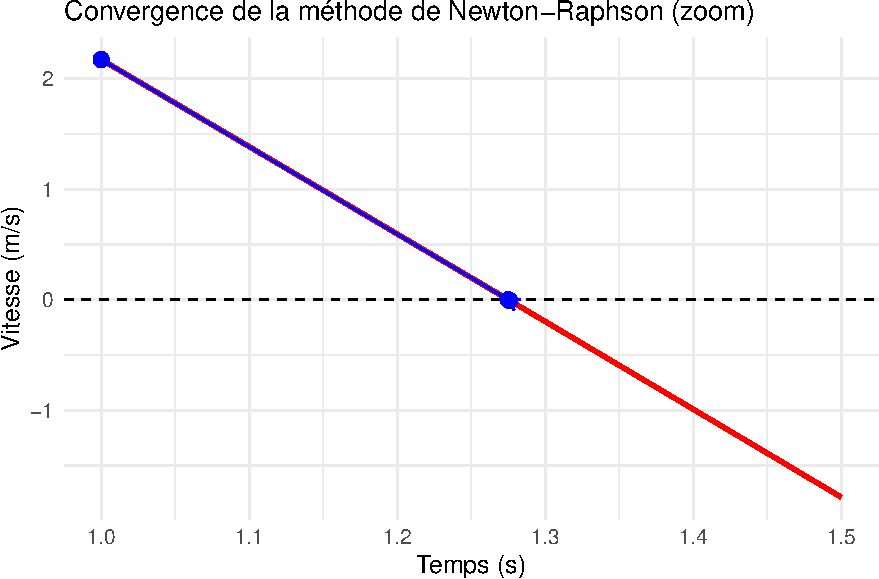
\includegraphics{theorie/pi/ballonmeteo_files/figure-pdf/fig-convergence-1.pdf}

}

\caption{\label{fig-convergence}Convergence de la méthode de
Newton-Raphson}

\end{figure}

\hypertarget{conclusion}{%
\subsection{Conclusion}\label{conclusion}}

La méthode de Newton-Raphson converge rapidement vers la solution : le
ballon atteint son altitude maximale après environ 1.275 secondes.

À cet instant, l'altitude du ballon est de 6.39 mètres.


\backmatter
\printbibliography


\end{document}
